%*******************************************************************************
%****************************** Second Chapter *********************************
%*******************************************************************************
\graphicspath{{Chapter2/Figs/}}

\chapter{Seasonal predictability of tropical storms in southern and central China}  

\section{Aims}
\begin{itemize}
	\item To explore the seasonal predictability of tropical storms in southern and central China
	\item Examine SST correlations up 17 months prior to the storm season
	\item Propose physical mechanisms by which SST offers seasonal predictability at long lead times

\end{itemize}

\section{Methods}
\subsection{Tropical storm data}

The Joint Typhoon Warning Center (JTWC) Best Track dataset provides the tropical storm data and was obtained from the IBTrACS database \cite{knapp2010international}. Any storms in the West Pacific that have a start time during the months of June to October and have a maximum intensity of least 34 knots (17 m/s, 38 mph) are selected. The dataset includes data on the position, maximum sustained winds, and minimum central pressure for every tropical cyclone globally at 6-hr intervals in UTC.

%The wind speed reported in this dataset is the maximum sustained wind over the 6 hourly time step?? also gusts?@!!! CHECK MSW used

\begin{figure}[h]
	\centering
	\noindent\includegraphics[width=20pc,angle=0]{China_domain.png}
	\caption{Domain marking landfalling storms in the southern and central China domain}\label{fig:landfall_domain}
\end{figure}

All of the storms that intersect a domain encompassing parts of southern and central China (figure \ref{fig:landfall_domain}) from 1958-2014 were chosen for further analysis. Although this includes data from the pre-satellite era, only landfalling storms are examined, and it is likely that these were recorded in the early periods.
%1958 is in the pre-satellite era, only landfalling storms are analysed and these were most likely recorded. The longer the time series the better.

The storms were separated into three categories based on maximum wind speed whilst within the specified domain based on the Saffir-Simpson Hurricane Scale (SSHS). Low intensity storms include tropical depressions and tropical storms (up to 63 knots, 32 m/s, 73 mph). Medium intensity include category one, and two storms from the SSHS (up to 95 knots, 49 m/s, 110 mph). High intensity storms were any that had a higher wind speed.

The standard temporal resolution of storm data is 6-hourly, however, at times there are missing time steps or additional data at a higher frequency. Storm data was interpolated onto a 6-hourly time period, for the calculation of accumulated cyclone energy (ACE), which is used as a proxy for damage. ACE is a value proportional to the energy of the system and is used to express the activity of individual TCs as well as entire TC seasons. The ACE of a season is the sum of the ACEs for each storm and takes into account the number, strength, and duration of all the tropical storms in the season. ACE is calculated by summing the squares of the maximum wind speed (knots) every 6 hours when the TC is within the domain of influence and is in 10\textsuperscript{4} knots\textsuperscript{2}. 

% outside maths mode use textsuperscript instead 10^{4}  	

\begin{equation}
ACE = 10^{-4}	 \sum v^2max
\end{equation}

Total ACE for the entire JJASO season for each year within the specified domain was calculated and will be referred to as ACE-JJASO. This a time series of one value for each season for 57 years (1958-2014).

Power Dissipation Index (PDI) is an alternative measure of tropical cyclone destructiveness, and uses the cube of the maximum wind speed rather than the square. PDI units are 10\textsuperscript{4} knots\textsuperscript{3}. PDI is like ACE but puts more emphasis on storm intensity.
%What is the advantage?
% This has shown to have some skill... cost of cyclones goes up with cube of the wind speed. (Southern reference in Emanuel 2005 Nature paper).
\begin{equation}
PDI = 10^{-4}	 \sum v^3max
\end{equation} 	 


\subsection{Large-scale environmental data}

The large-scale environment data comes from various reanalysis datasets (\ref{t1}). The NCEPNCAR reanalysis \citep{kalnay1996ncep} and JRA-55 reanalysis \citep{kobayashi2015jra} provide the atmospheric data. The NCEPNCAR data extends back until 1948 and has been used in numerous previous studies examining the statistical relationship between the large-scale environment and tropical storm activity. JRA-55 is a more recent reanalysis produced by the Japanese Meteorological Agency (JMA) and is also at higher resolution than the NCEPNCAR dataset.

The SST data from Extended Reconstructed SST (ERSSTv4) dataset \citep{huang2015extended} covers over 150 years, starting in 1854. With the increased availability of sub-surface ocean observations, there are recent reanalyses that included data on ocean heat content. The NCEPCFSR coupled reanalysis \citep{saha2010ncep} provides the tropical cyclone heat potential (TCHP) data, which is the ocean heat content down to the 26$^0$C isotherm, however, data is only available from 1979 - 2010. This TCHP data also only extends to areas with tropical cyclone activity. An alternative product for data on the deeper ocean is the ORSA4 reanalysis \citep{balmaseda2013evaluation}, produced by ECMWF. Ocean heat content (OHC) data to a variety of depths is available, the shallowest being 100m, which was used.

% http://tex.stackexchange.com/questions/47324/superscript-outside-math-mode

\begin{table}[h]
	\caption{Details of data used}\label{t1}
	\begin{center}
		\begin{tabular}{cccc}
			\hline\hline
			$Dataset$ & $Variable$ & $Resolution (grid points)$ & $Years$ \\
			\hline
			JRA-55 & *atmosphere & T319 L60 1.25$^0$ & 1958-2013 \\ %% $ $ is math mode - put this around the bits that are not text
			\citep{kobayashi2015jra} & & (145 x 288) & \\
			NCEPNCAR & *atmosphere & T62 L28 2.5$^0$ & 1948-2014 \\
			\citep{kalnay1996ncep} & & & \\
			ERSSTv4 & SST & 2$^0$ & 1970-2014 \\
			\citep{huang2015extended} & & (89 x 180) & \\
			NCEPCFSR & TCHP & T382 L64 0.5x0.5$^0$ & 1979-2009  \\
			\citep{saha2010ncep} & & & \\
			ORSA4 & OHC & Refined at Tropics 0.3x0.3$^0$ & 1958-2009  \\
			\citep{balmaseda2013evaluation} & & (180 x 360) & \\
			
			\hline
		\end{tabular}
	\end{center}
\end{table}

% nCEP-CFSR(38km)
* atmosphere included mean sea level pressure, relative vorticity, relative humidity, u wind, v wind, precipitable water.

Monthly means of the variables were created, along with monthly tendencies and means of multiple months, e.g. JFM, MAM.


\subsection{Correlation analysis}

To produce correlation maps, the ACE or frequency time series was correlated with the time series of the variable at each grid point. The Pearson R value is a measure of the linear dependence between two variables, giving a value between plus 1 and minus 1 inclusive, where 1 is total positive linear correlation and minus 1 is total negative linear correlation.

The Pearson product moment correlation coefficient is calculated as follows:
%https://data.vanderbilt.edu/biosproj/CI2/corr.tex

$r = \frac{\Sigma(x_i - \bar{x})(y_i - \bar{y})}{\sqrt{\Sigma(x_i - \bar{x})^2\Sigma(y_i - \bar{y})^2}}$

The Pearson R value gives information on the direction and strength of correlation (\ref{tcorrs}). % with 0.3-0.4 OR 0.5 weak then moderate then strong >0 being very strong, in between is moderate.

\begin{table} % remove [h] and sits in right place
	\caption{Interpretation of Pearson R correlation coefficient}\label{tcorrs}
	\begin{center}
		\begin{tabular}{cc}
			\hline\hline
			Correlation coefficient R & Correlation strength \\
			\hline
			.70 or higher & very strong  \\ 
			.40 to +.69 & strong \\ 
			.30 to +.39 & moderate  \\
			.20 to +.29 & weak \\
			
			\hline
		\end{tabular}
	\end{center}
\end{table}


This coefficient is accompanied by a p-value, which is a number between 0 and 1 representing the probability that this data would have arisen by chance. A p-value of 0.01 is ‘highly significant’ and a value of 0.05 is 'significant'.

%R\textsuperscript{2} is often used. This value describes how much variability of one variable is explained by another.

%nB WHAT ABOUT SST REANALYSES ERRORS PRE SATELITE 1980?? (deser et al)
%nB PDO is an eof, - JUST A RESULT of something?

For each grid point where variable data was available, the time series was correlated against ACE-JJASO. For example, figure \ref{fig:corr_graph} shows the two time series for one grid point and their correlation. %This point is located at lon 320 and lat -60 and so on the maps the correlation value will be marked as ..... see the following figures.


\begin{figure}
	\centering
	\noindent\includegraphics[width=20pc,angle=0]{SST_ACE_corr.png}
	\caption{Correlation of ACE(10$^4$kt$^2$) and SST($^0$C) time series at one grid point. Pearson R correlation and p-value shown.}\label{fig:corr_graph}
\end{figure}



%%%%%%%%%%%%%%%%%%%%%%%%%%%%%%%%%%%%%%%%%%%%%

\section{Results}

\subsection{Storm activity within specified domain}

Storm activity was determined by storm frequency, ACE and PDI. In the low intensity group (tropical storms and tropical depressions), there are 204 storms over the 57 year period. There are 177 in the medium intensity (categories 1, and 2), and 63 in the high intensity (categories 3, 4 and 5).

ACE and PDI were calculated in two ways. Firstly, by just using the storm time steps whilst within the domain (ACE domain), and second, by calculating the ACE along the entire storm track (ACE / PDI entire) (figure \ref{fig:landfall_domain}). These different ACE and PDI values are correlated with each other and the frequency values (\ref{tcorrs2}).


\begin{table}
	\centering
	\caption{Pearson R correlation coefficient for 57 year time series. Bold indicates p<0.01. Bold star indicates p<0.05}\label{tcorrs2}
	\begin{tabular}{ |c|c|c|c|c| } 
		\hline
		 & ACE(entire) & PDI(domain) & PDI(entire) & count \\
		\hline
		\multirow{3}{5em}{ACE(domain)} & \textbf{0.43} & \textbf{0.99} & 0.25 & \textbf{0.79} \\ 
		& \textbf{0.73} & \textbf{0.99} & \textbf{0.61} & \textbf{0.86}  \\ 
		& \textbf{0.89} & \textbf{0.99} & \textbf{0.87} & \textbf{0.93}  \\ 
		\hline
		\multirow{3}{5em}{ACE(entire)}  & - & \textbf{0.41}* & \textbf{0.96} & \textbf{0.52} \\ 
		 & - & \textbf{0.72} & \textbf{0.98} & \textbf{0.79}  \\ 
		 & - & \textbf{0.88} & \textbf{0.99} & \textbf{0.96}  \\ 
		\hline
		\multirow{3}{5em}{PDI(domain)} & - & - & 0.24 & \textbf{0.92} \\ 
		 & - & - & \textbf{0.61} & \textbf{0.84}  \\ 
		 & - & - & \textbf{0.88} & \textbf{0.92}  \\ 
		\hline
		\multirow{3}{5em}{PDI(entire)}  & - & - & - & \textbf{0.34}* \\ 
		 & - & - & - & \textbf{0.69}  \\ 
		 & - & - & - & \textbf{0.93}  \\ 
		\hline
%		\multirow{3}{4em}{count} & - & - & - & - & - \\ 
%		& - & - & - & - & -  \\ 
%		& - & - & - & - & -  \\ 
%		\hline
	\end{tabular}
\end{table}


When comparing the 'entire' together and 'domain' together, the ACE and PDI time series have a high correlation with each other (more than 0.95), as equations x show that they are just a factor of something. Count is larger than 0.7 for all but a few low category correlations. The remaining comparisons between the domain and entire are generally significant at the 99th percentile, with increasing R values with increasing category.Results will focus on ACE and count, in domain.

Annual storm frequency shows interannual variation across all categories (figure \ref{fig:counts}).

\begin{figure}
	\subfloat[Low]{\includegraphics[width=1.9in]{ACE_count_63.png}} 
	\subfloat[Medium]{\includegraphics[width=1.9in]{ACE_count_95.png}} % Y:/Code_Data/Chapter1/Plots_new/Charts
	\subfloat[High]{\includegraphics[width=1.9in]{ACE_count_plus.png}} 
	\caption{Time series of ACE (domain and entire) and frequency for each category. a) low, b) medium, c) high }\label{fig:counts}
\end{figure}

Remain on plots from lifetime to entire and redo or remove the correlation values
%204, 209, 31
%204, 177, 63

Make it clear that all results use ACE in domain and count of anything that has intersected the domain.

\subsection{Correlation between storm activity and large-scale variables}

%% Look at SST variability within each box. How variable is SST on an interannual time scale?

The following maps show the Pearson R correlation values between the environmental variable at each grid point and ACE-JJASO and count-JJASO over the available period from 1958. This is 57 years for sst (to 2014), 56 years for atmospheric variables (to 2013) and 52 years for OHC (to 2009). The stippled areas are significant at the 95th percentile (p\textless0.05). Solid black contour lines are shown when the Pearson R coefficient is less than -0.3 and more than 0.3.


\subsubsection{SST and OHC}

This first section examines the relationship between the ocean (SST and OHC) with storm activity.
%	\subfloat[1a]{\includegraphics[width=2.4in]{Y:/Code_Data/Chapter1/Plots_new/Corr_maps_final/ACE/inpoly/sst_curr_JJASO&ACEJJASO63inpolycorr_train.png}}
	
\begin{figure}
	\centering
	\subfloat[ACE:low]{\includegraphics[width=2.6in]{sst_curr_JJASO&ACEJJASO63inpolycorr_total.png}}
	\subfloat[Count:low]{\includegraphics[width=2.6in]{sst_curr_JJASO&countJJASO63inp_intcorr_total.png}}
	\subfloat[ACE:medium]{\includegraphics[width=2.6in]{sst_curr_JJASO&ACEJJASO95inpolycorr_total.png}}
	\subfloat[Count:medium]{\includegraphics[width=2.6in]{sst_curr_JJASO&countJJASO95inp_intcorr_total.png}}
	\subfloat[ACE:high]{\includegraphics[width=2.6in]{sst_curr_JJASO&ACEJJASOplusinpolycorr_total.png}}
	\subfloat[Count:high]{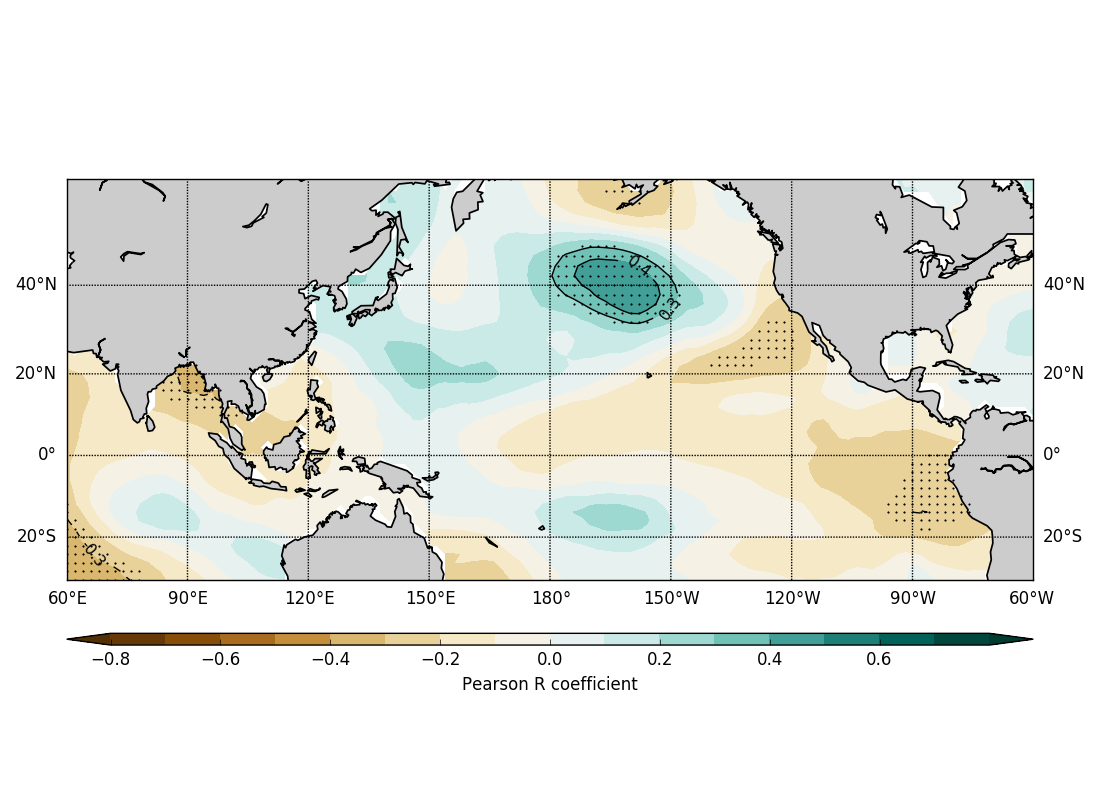
\includegraphics[width=2.6in]{sst_curr_JJASO&countJJASOplusinp_intcorr_total.png}}
	\subfloat[ACE:all]{\includegraphics[width=2.6in]{sst_curr_JJASO&ACEJJASOallcatsinpolycorr_total.png}}
	\subfloat[Count:all]{\includegraphics[width=2.6in]{sst_curr_JJASO&countJJASOallcatsinp_intcorr_total.png}} % Y:/Code_Data/Chapter1/Plots_new/Corr_maps_final/count/inp_int/sst/  
	% Y:/Code_Data/Chapter1/Plots_new/Corr_maps_final/ACE/inpoly/sst/
	
	\caption{SST-JJASO correlated with (1) and ACE and (2) count over the period 1958-2014. a) Low (tropical storms and tropical depressions). b) Medium (categories 1,2) c) High (categories 3, 4, 5) d) a. Stippling indicates grid points with significant correlation at the 95th percentile} \label{fig:corr_JJASO} 
\end{figure} 

The correlation maps in column 1 (SST correlated with ACE) are similar to those in column 2 (SST correlated with count), suggesting that the relationship with SST is dominated by frequency of storms rather than intensity.

The plots in figure \ref{fig:corr_JJASO} show that there are notable differences between the relationship with SST and tropical storm activity for different intensity storms. For the low intensity storms, there is an area of significant positive correlation in the Philippine Sea, extending northwards encompassing the East China Sea and eastwards to the east of Japan (figure \ref{fig:corr_JJASO},2a). This in the the region of the Kuroshio currents, where warm water is advected .....The storms during the season pass over this water in the Philippines / East China Sea, to make landfall in the selected domain. When the SST here is anomalously warm, there are an increased number of tropical storms and tropical depressions making landfall here and vice versa.

For the medium intensity storms, there is a significant negative correlation in the central equatorial Pacific (figure \ref{fig:corr_JJASO}b). For the intense storms (figure \ref{fig:corr_JJASO},c), a maximum correlation of between 0.4 and 0.5 is apparent in the northern North Pacific. No regions of significant correlation are observed across all of the different categories.
%There is a negative correlation in the Southern Indian Ocean and South China Sea, and Bay of Bengal as well as eastern equatorial Pacific. 
The negative correlations in the medium and intense storms in the equatorial Pacific are likely to be El Nino, which varies on an interannual time scale. In both cases, the correlation is negative, suggesting that during El Nino (central for medium and EPAC for intense), there are fewer storms making landfall in the selected domain.

Figures 1d and 2d are the relationship with all storms. The largest area of significance is the equatorial Pacific, with a negative correlation. As might be expected, these plots (1d and 2d) show the largest difference, as there are more storms in total being analysed in these plots and ...
Future correlation maps will show the relationship with count, as the observations are subject to less error than wind that goes into the ACE calculation.
%When the sum of ACE for all categories is plotted as above (not shown), .........


\begin{figure}
	\centering
	\noindent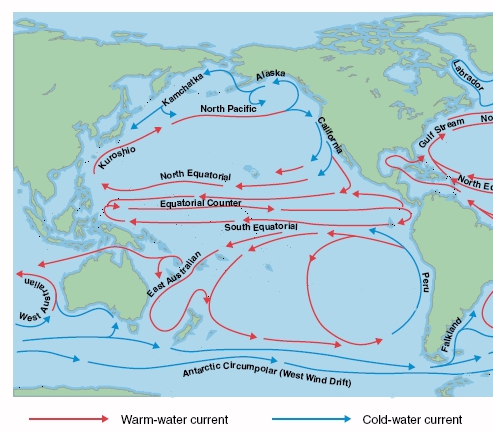
\includegraphics[width=24pc,angle=0]{ocean_currents2_cut.png}
	\caption{Ocean currents showing Kurushio. Source: \citep{kuroshio}}\label{fig:kuroshio}
\end{figure}


\begin{figure}
	\centering % Y:/Code_Data/Chapter1/Plots_new/Corr_maps_final/count/inp_int/sst/
	%\subfloat[1a]{\includegraphics[width=2.4in]{Y:/Code_Data/Chapter1/Plots_new/Corr_maps/ACE/inpoly/prev_sst_JFM&ACEJJASO63inpolycorr_train.png}} 
	\subfloat[2a]{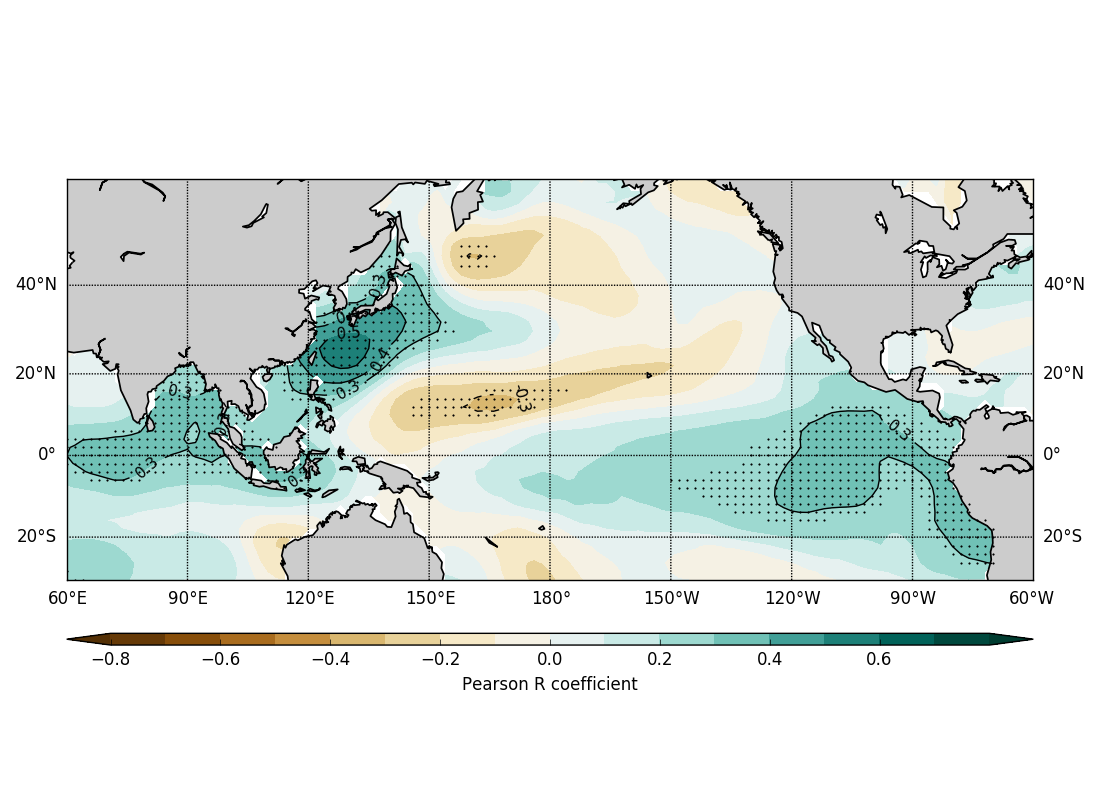
\includegraphics[width=2.6in]{sst_prev_JFM&countJJASO63inp_intcorr_total.png}}
	%\subfloat[1b]{\includegraphics[width=2.4in]{Y:/Code_Data/Chapter1/Plots_new/Corr_maps/ACE/inpoly/prev_sst_JFM&ACEJJASO95inpolycorr_train.png}}
	\subfloat[2a]{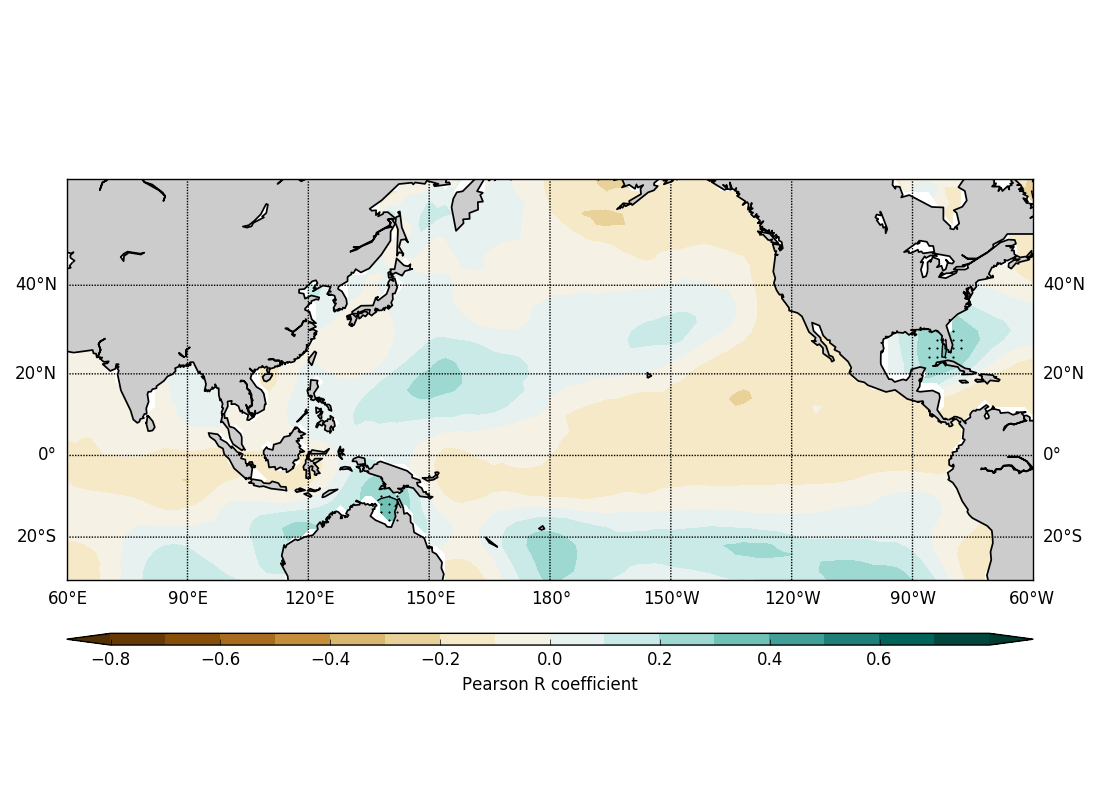
\includegraphics[width=2.6in]{sst_prev_JFM&countJJASO95inp_intcorr_total.png}}
	%\subfloat[1c]{\includegraphics[width=2.4in]{Y:/Code_Data/Chapter1/Plots_new/Corr_maps/ACE/inpoly/prev_sst_JFM&ACEJJASOplusinpolycorr_train.png}}
	\subfloat[2a]{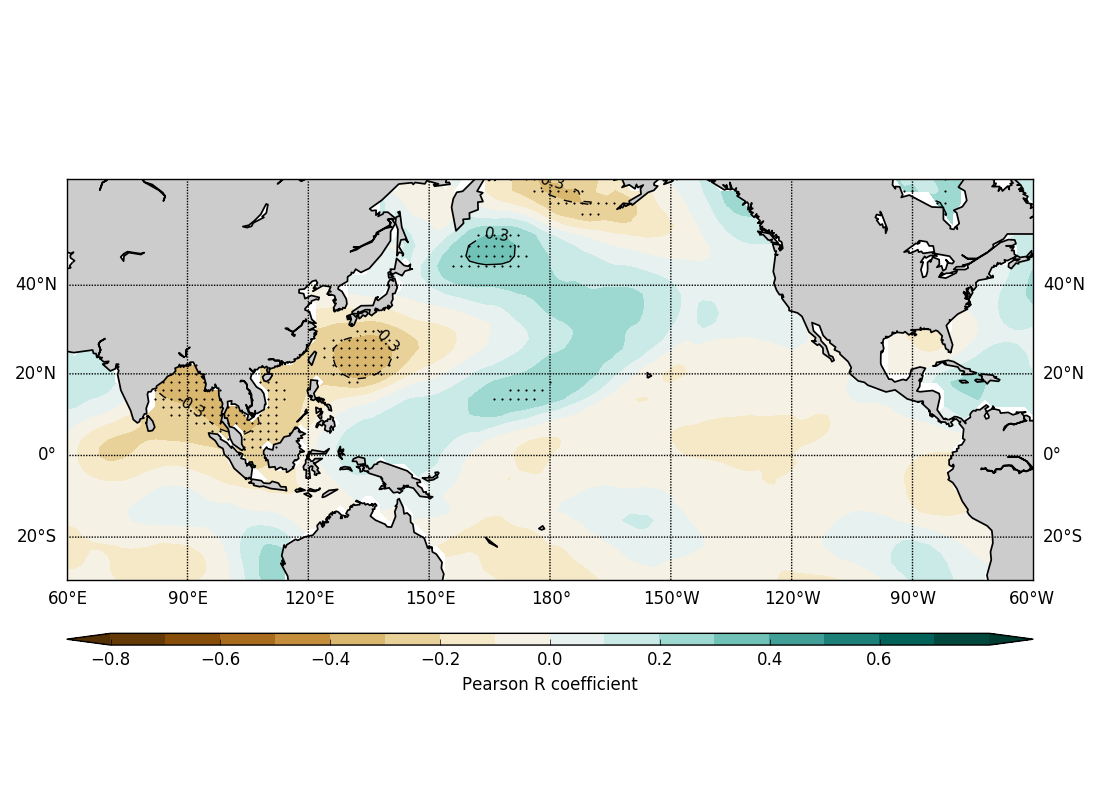
\includegraphics[width=2.6in]{sst_prev_JFM&countJJASOplusinp_intcorr_total.png}}
	%\subfloat[1d]{\includegraphics[width=2.4in]{Y:/Code_Data/Chapter1/Plots_new/Corr_maps/ACE/inpoly/prev_sst_JFM&ACEJJASOallcatsinpolycorr_train.png}}
	\subfloat[2a]{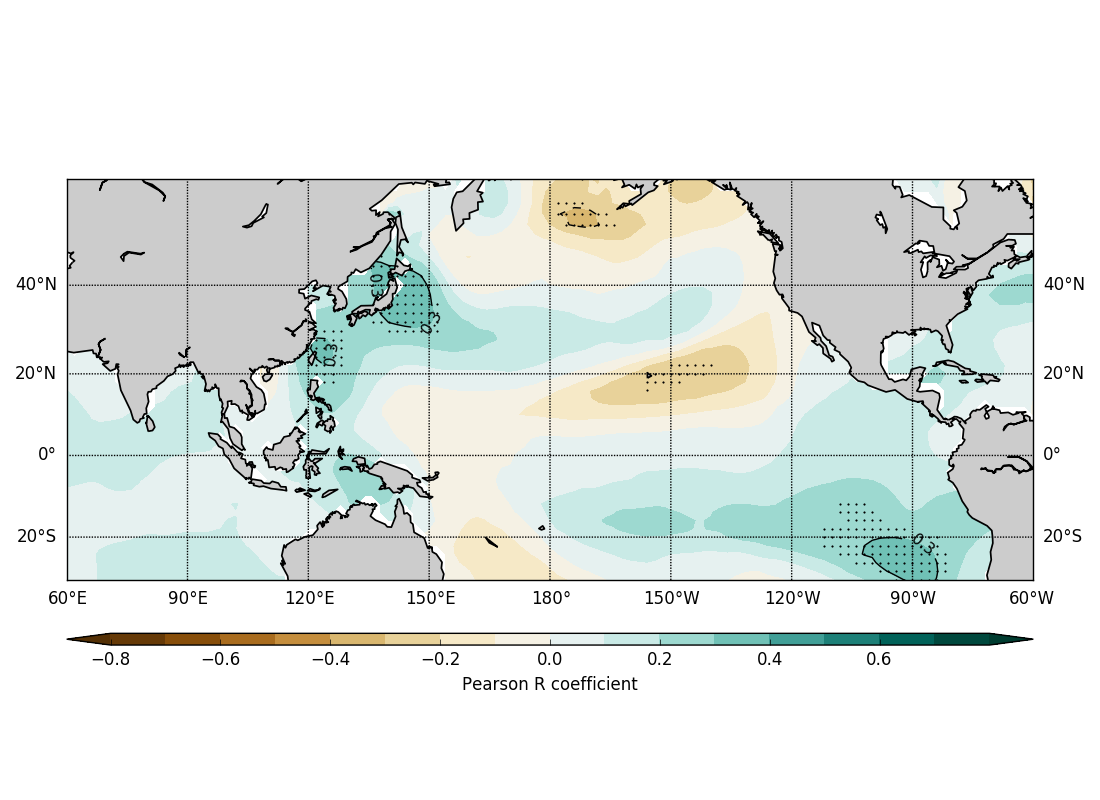
\includegraphics[width=2.6in]{sst_prev_JFM&countJJASOallcatsinp_intcorr_total.png}}
	\caption{SST-JFM-1 correlated with count over the period 1958-2014. a) Low (tropical storms and tropical depressions). b) Medium (categories 1,2) c) High (categories 3, 4, 5) d) All storms. Stippling indicates grid points with significant correlation at the 95th percentile} \label{fig:corr_prevJFM} 
\end{figure} 

When correlating ACE-JJASO and count-JJASO with SSTs in the year prior to the storm season, the most consistent and significant signal is seen in JFM ('JFM-1') off the east coast of mainland China, in the East China Sea (figure \ref{fig:corr_prevJFM}) and in the Bay of Bengal (particularly when correlating against count), parts significant in the South China Sea. There is a striking anti-correlation between the results for the low intensity storms (figure \ref{fig:corr_prevJFM}, a) and the high intensity storms (figure \ref{fig:corr_prevJFM}, c) in this region. For the weakest storms, there is a positive correlation with SST, but for the most intense storm this correlation is negative. Both categories show significance at the 95th percentile in this region.  Alongside this region, there are correlations of the opposite sign extending northeastwards towards the Aleutian Islands and also at around 10-20N and to the east of this main site.

The lag between these anomalies and the storm activity is approximately 18 months.

For the medium intensity storms, however, there is no significant correlation with SST in this region (figure \ref{fig:corr_prevJFM}, b). %The highest Pearson R correlation value is around 0.5, giving an R\textsuperscript{2} of 0.25. This suggests that 25\% of the variability in ACE or count each year is explained by the SST in this region in the previous JFM. 

The low intensity storms also have a large region of positive correlation in the eastern equatorial Pacific. During JFM, if there is an El Nino situation, the anomalous sea surface temperature in this region can still be large and decreasing? This indicates that in the year following an El Nino i.e. 15 months later?, there are increased number of tropical storms and depressions in the domain.


%correlated because trend and sst and ace both increasing? or because time series variability is correlated on interannual timescale?
%pLOT storms that do not intersect and see how they miss the domain - above or below or stay out at sea?

In the JFM just before the JJASO season, the signal in this region for the intense storms has largely disappeared although some significance re3mains in the Bay of Bengal for the weak storms. (not shown).

%\begin{figure}
%	\centering
%	\subfloat[2a]{\includegraphics[width=2.6in]{Y:/Code_Data/Chapter1/Plots_new/Corr_maps_final/count/inp_int/sst/sst_curr_JFM&countJJASO63inp_intcorr_total.png}}
%%	\subfloat[2b]{\includegraphics[width=2.4in]{Y:/Code_Data/Chapter1/Plots_new/Corr_maps/count/inp_int/curr_sst_JFM&countJJASO95inp_intcorr_train.png}}
%	\subfloat[2a]{\includegraphics[width=2.6in]{Y:/Code_Data/Chapter1/Plots_new/Corr_maps_final/count/inp_int/sst/sst_curr_JFM&countJJASOplusinp_intcorr_total.png}}
%	
%	\caption{SST-JFM correlated with count-JJASO for within the domain over the training period 1958-2007. a. Tropical storms and tropical depressions. b. Categories 3, 4 and 5. Stippling shows grid points with significant correlation at 95th percentile} \label{fig:corr_currJFM} 
%	\end{figure} 

\begin{table}[h]
	\caption{Coordinates of regions}\label{tregion_coors}
	\begin{center}
		\begin{tabular}{ccc}
			\hline\hline
			Region & Coordinates & Signal\\
			\hline
			East China Sea & 0-40N, 120-140E,  & JJASO, Low, positive  \\ 
			East China Sea2 & 15-35N, 120-140E,  & JFM-1, low, positive. JFM-1, high, negative \\ 
			Bay of Bengal & 5-20N, 80-100E & JJASO, high, negative. JFM-1, low, positive. JFM-1, high, positive \\ 
			NNPac & 32-47N, 180-150W & JJASO, high, positive  \\ 
			Kuroshio & 35-47N, 145-175E & JJASO, Low, positive, JFM-1, low, negative. JFM-1, high, positive  \\ 
			Oyashio & 40-53N, 155-170E & JFM-1, low, negative. JFM-1, high, positive  \\
			Anew & 10-20N, 160-180E & JFM-1, low, negative. JFM-1, high, positive   \\ 
						
			\hline
		\end{tabular}
	\end{center}
\end{table}


This region of interest will be further examined, concentrating on the weak and intense storms only.

Figure \ref {fig:SCS} shows the domain where these opposing strong correlations are apparent. 
\begin{figure} % remove [h] and this appeared in the correct place
	\noindent\includegraphics[width=26pc,angle=0]{corr_regions.png} % Y:/Code_Data/Chapter1/Plots_new/Maps/
	\caption{Regions of high correlations}\label{fig:SCS}
\end{figure}

\begin{figure} % remove [h] and this appeared in the correct place
	\noindent\includegraphics[width=26pc,angle=0]{nino_regions.png}
	\caption{Nino regions}\label{fig:nino}
\end{figure}

% check means are 50 years or 57 years?
Figure \ref{fig:SST_JJASO} shows that during the tropical cyclone season (JJASO), there is a large region of warm SSTs, well above the 26.5$^0$C proposed threshold for genesis (section \ref{ocean}). The standard deviation of the SSTs across the period in both JJASO and JFM shows the most variation year to year in the equatorial Pacific, where the El Nino phenomenon has a signal and this shows significant interannual variability. %Off the east coast of Asia and into the Bay of Bengal, the standard deviation is 0.6 to 0.3 C??

\begin{figure} % remove [h] and this appeared in the correct place
	\subfloat[a]{\includegraphics[width=3.5in]{sst_JJASO_mean.png}} % Y:/Code_Data/Chapter1/Plots_new/Charts/
	\subfloat[b]{\includegraphics[width=3.5in]{sst_JJASO_std.png}} 
	\subfloat[c]{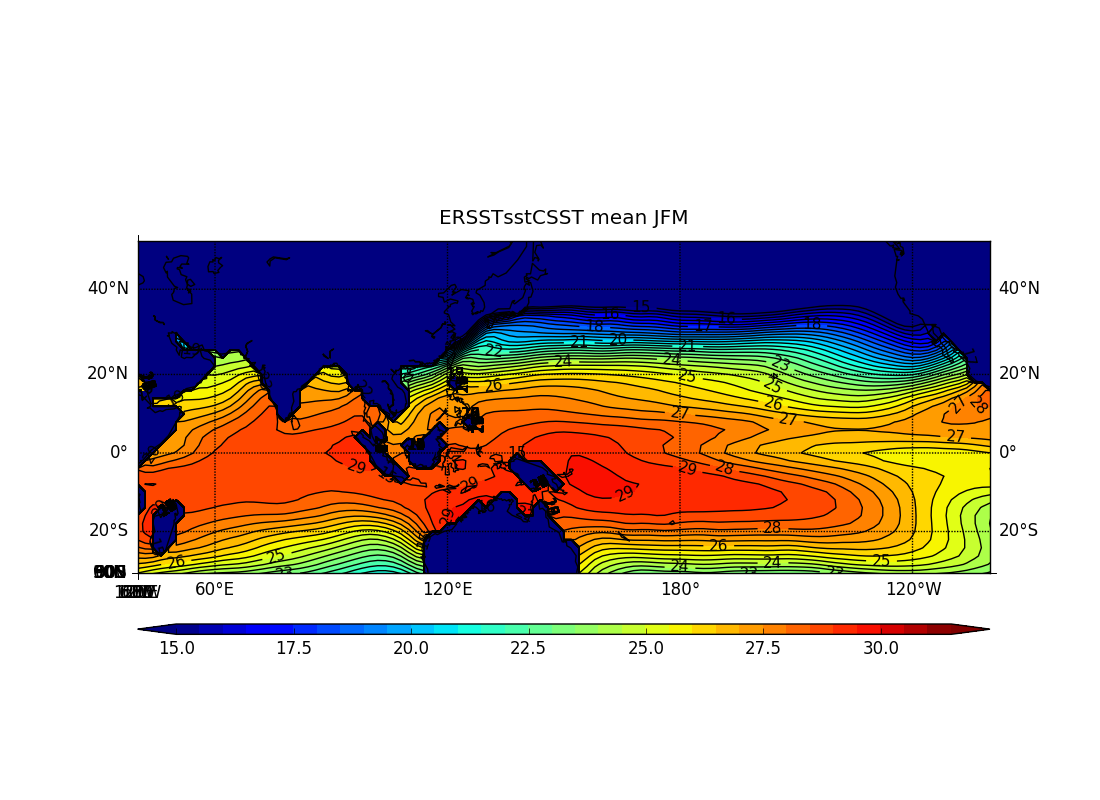
\includegraphics[width=3.5in]{sst_JFM_mean.png}} 
	\subfloat[c]{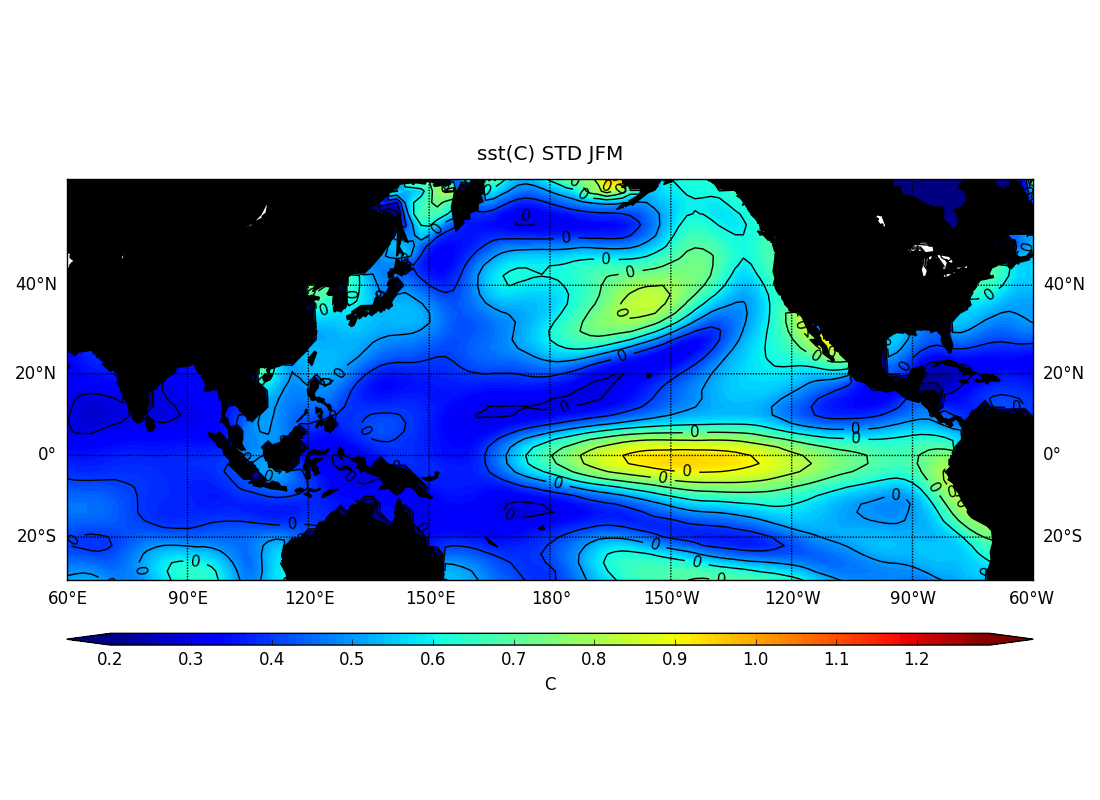
\includegraphics[width=3.5in]{sst_JFM_std.png}} 
	
	\caption{SST climatology. (a) JJASO mean (b) JJASO standard deviation (c) JFM standard deviation. The standard deviations are of the JJASO mean across the 50 year training period.}\label{fig:SST_JJASO}
\end{figure}

Unlike in the North Atlantic, where tropical cyclogenesis is restricted by the cooler SSTs, in the West Pacific, there is a large region where SSTs are not the restricting factor. Therefore, something else at play? Also steering is important.
This region of warm water migrates north or south depending on the season. Warm pool to the west of the basin and cooler upwelling water to the east.

This period examined from 1958 and is likely to contain decadal signals. To assess whether the signals seen in figures \ref{fig:corr_JJASO} and \ref{fig:corr_prevJFM} are stable throughout the period, the results have been broken down into three periods that line up with different Pacific Decadal Oscillation (PDO) phases (cold, warm and mixed) (figure \ref{fig:PDO_time}, table \ref{tperiods}).

% 	\begin{figure}
% 		\noindent\includegraphics[width=35pc,angle=0]{Y:/Code_Data/PDO/Figure_PDO-01.jpg}\\
% 		\caption{The Pacific Decadal Oscillation( (PDO) Index. From https://www.nwfsc.noaa.gov/research}\label{fig:PDO_time}
% 	\end{figure}


\begin{figure}
	\centering
	\noindent\includegraphics[width=20pc,angle=0]{PDO_5814_filled.png} % Y:/Code_Data/Chapter1/Plots_new/Charts
	\caption{The Pacific Decadal Oscillation Index}\label{fig:PDO_time}
\end{figure}

\begin{table}[h]
	\caption{Periods}\label{tperiods}
	\begin{center}
		\begin{tabular}{ccc}
			\hline\hline
			Years & Number of years & PDO state \\
			\hline
			1958-1975 & 18 & cold  \\ 
			1976-1997 & 22 & warm  \\ 
			1998-2014 & 17 & mixed  \\ 
			
			\hline
		\end{tabular}
	\end{center}
\end{table}


The following figures show the correlation maps for each category for the three different periods \ref{tperiods}. Column 1 is 1958-1975 (cold), 2 is 1976-1997 (warm), and 3 is 1998-2014 (mixed). 


\begin{figure}
	\centering % Y:/Code_Data/Chapter1/Plots_new/Corr_maps_final/count/inp_int/sst/
	
	\subfloat[2a]{\includegraphics[width=1.8in]{sst_curr_JJASO&countJJASO63inp_intcorr_early.png}}
	\subfloat[2a]{\includegraphics[width=1.8in]{sst_curr_JJASO&countJJASO63inp_intcorr_mid.png}}
	\subfloat[2a]{\includegraphics[width=1.8in]{sst_curr_JJASO&countJJASO63inp_intcorr_late.png}}
	
%	\subfloat[2a]{\includegraphics[width=1.8in]{Y:/Code_Data/Chapter1/Plots_new/Corr_maps_final/count/inp_int/sst/sst_curr_JJASO&countJJASO95inp_intcorr_early.png}}
%	\subfloat[2a]{\includegraphics[width=1.8in]{Y:/Code_Data/Chapter1/Plots_new/Corr_maps_final/count/inp_int/sst/sst_curr_JJASO&countJJASO95inp_intcorr_mid.png}}
%	\subfloat[2a]{\includegraphics[width=1.8in]{Y:/Code_Data/Chapter1/Plots_new/Corr_maps_final/count/inp_int/sst/sst_curr_JJASO&countJJASO95inp_intcorr_late.png}}
% Y:/Code_Data/Chapter1/Plots_new/Corr_maps_final/count/inp_int/sst/
	
	\subfloat[2a]{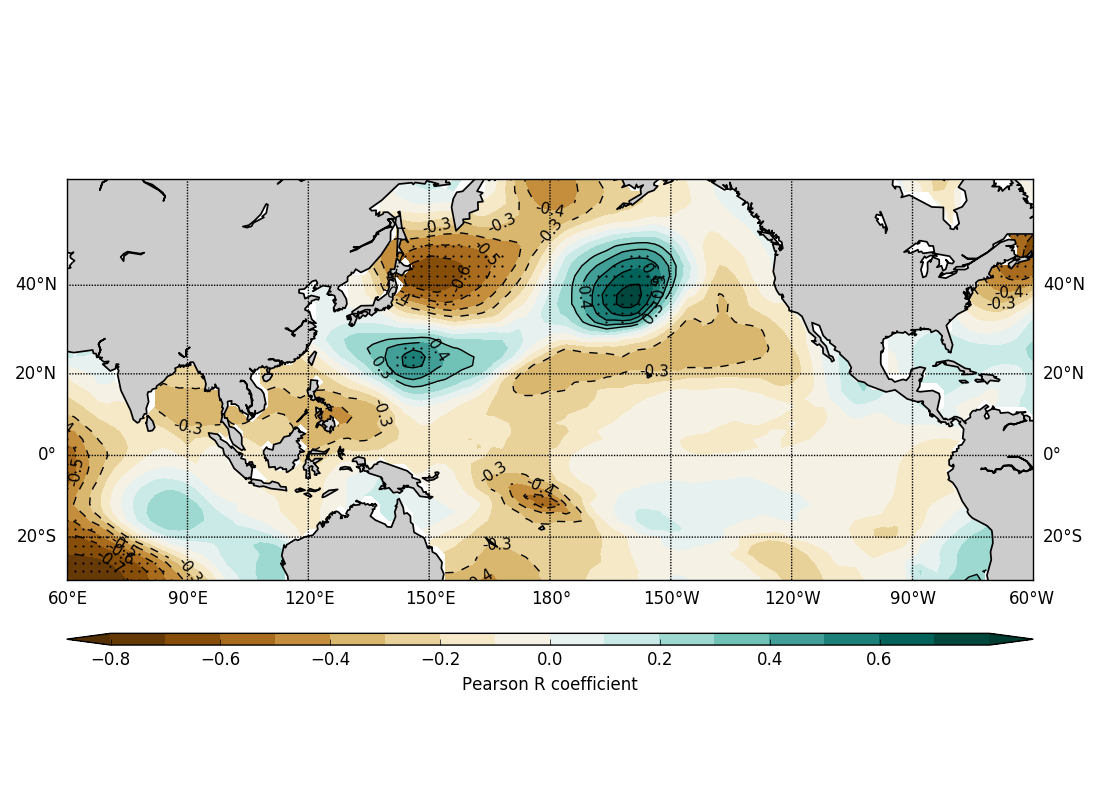
\includegraphics[width=1.8in]{sst_curr_JJASO&countJJASOplusinp_intcorr_early.png}}
	\subfloat[2a]{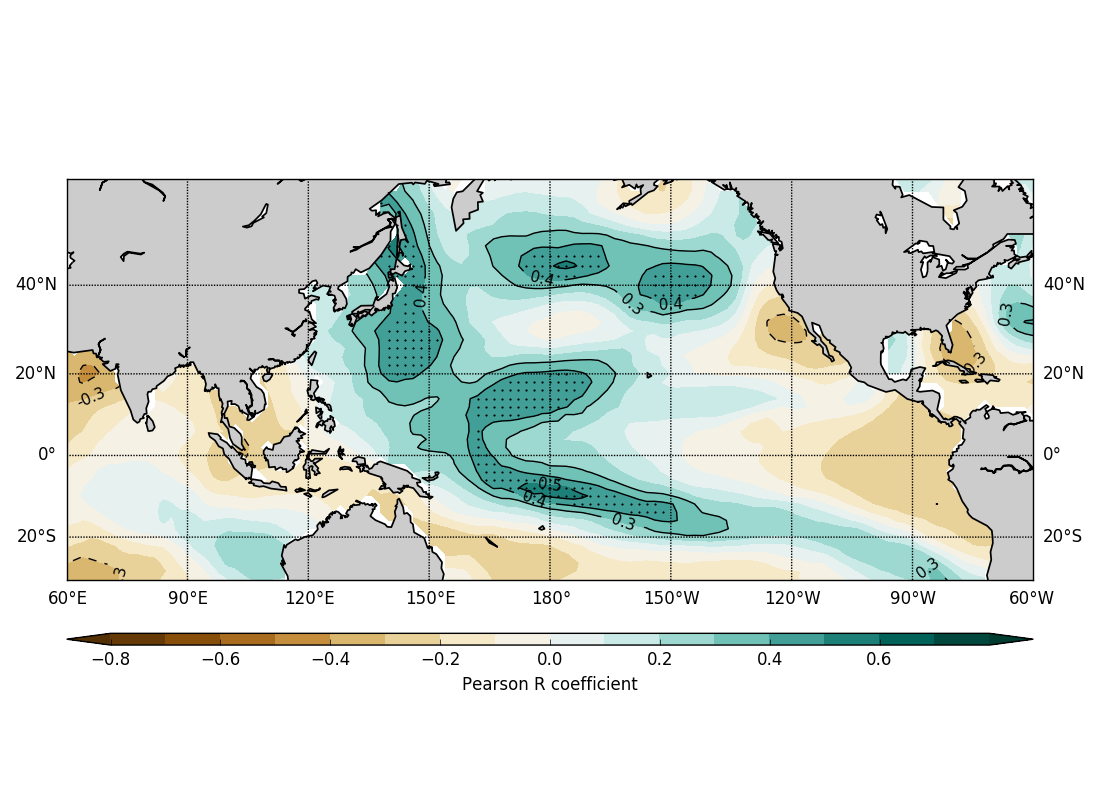
\includegraphics[width=1.8in]{sst_curr_JJASO&countJJASOplusinp_intcorr_mid.png}}
	\subfloat[2a]{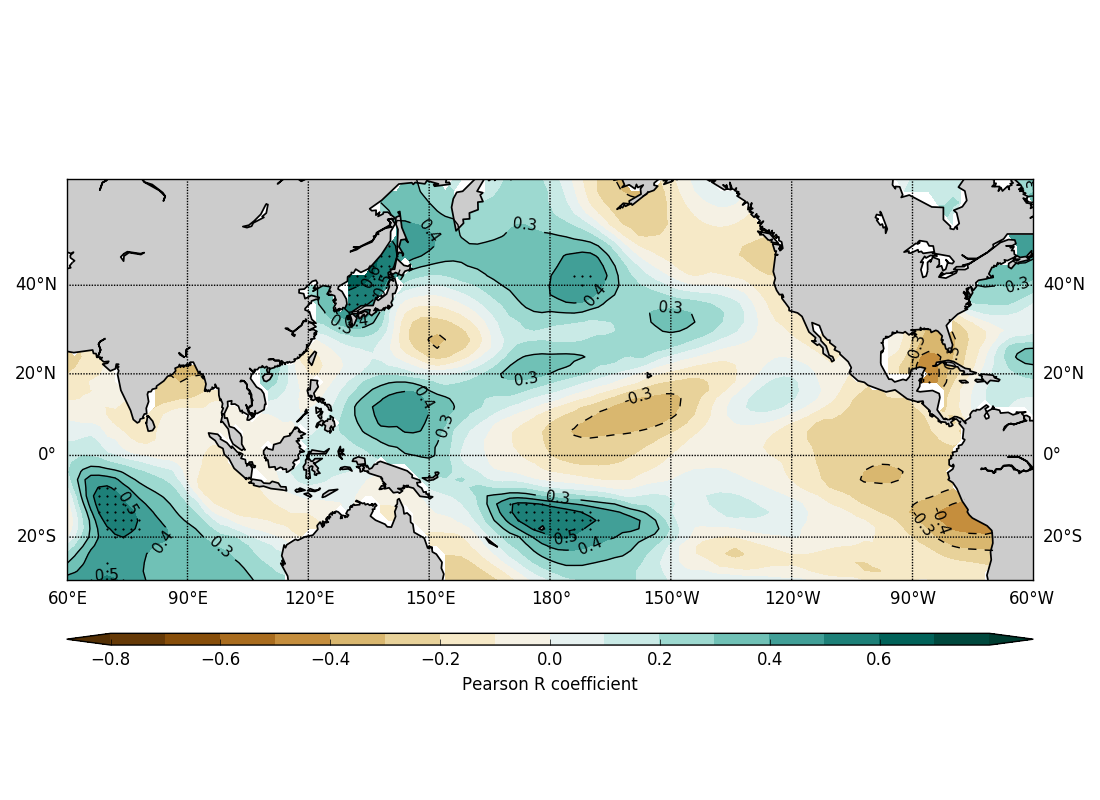
\includegraphics[width=1.8in]{sst_curr_JJASO&countJJASOplusinp_intcorr_late.png}}
	\caption{SST-JJASO correlated with count-JJASO for within the domain for 1958-1975 (1), 1976-1997 (2), 1998-2014 (3). a. Tropical storms and tropical depressions. b. Categories 1,2 c. Categories 3, 4, 5.  Stippling shows grid points with significant correlation at 95th percentile} \label{fig:corr_JJASO_periods} 
\end{figure} 

sort this out:

In JJASO, the positive correlation seen to the east of Japan is strong in the middle (warm period), with no significant correlations in the other periods. The positive correlation in the Philippine Sea and East China Sea are present in less coherent regions and not as strong a correlation (figure \ref{fig:corr_JJASO_periods}, 2a). The final (mixed) phase has no areas of significant correlation. 
 There are also areas of significant correlation across the equatorial Pacific  -check.

For the high intensity storms, the positive correlation at approximately 160W and 40N is apparent in all periods, strongest during the cool phase when it has a dipole with the Kuroshio region. (refer to PDO phase diagram in intro).
%cHECK WHETHER PDO YEARS SHOULD BE ADJUSTED BY ONE WHEN LOOKING AT PREV YEAR

\begin{figure}
	\centering % Y:/Code_Data/Chapter1/Plots_new/Corr_maps_final/count/inp_int/sst/
	
	\subfloat[2a]{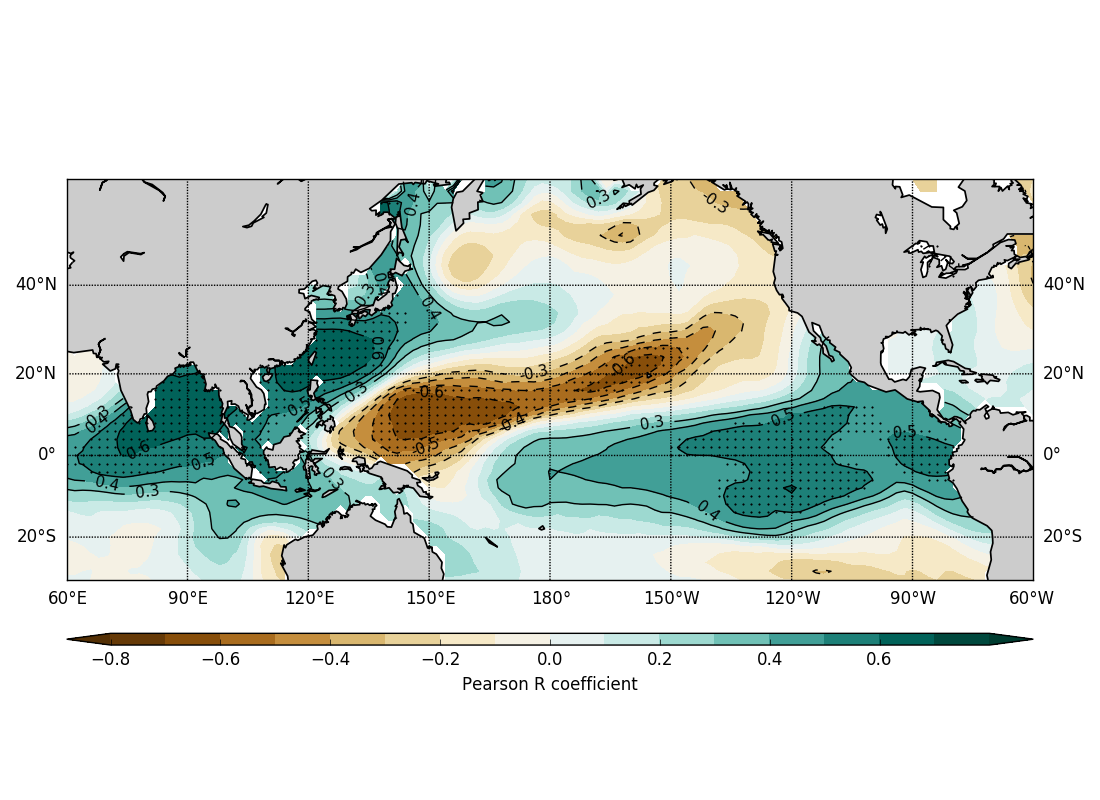
\includegraphics[width=1.8in]{sst_prev_JFM&countJJASO63inp_intcorr_early.png}}
	\subfloat[2a]{\includegraphics[width=1.8in]sst_prev_JFM&countJJASO63inp_intcorr_mid.png}}
	\subfloat[2a]{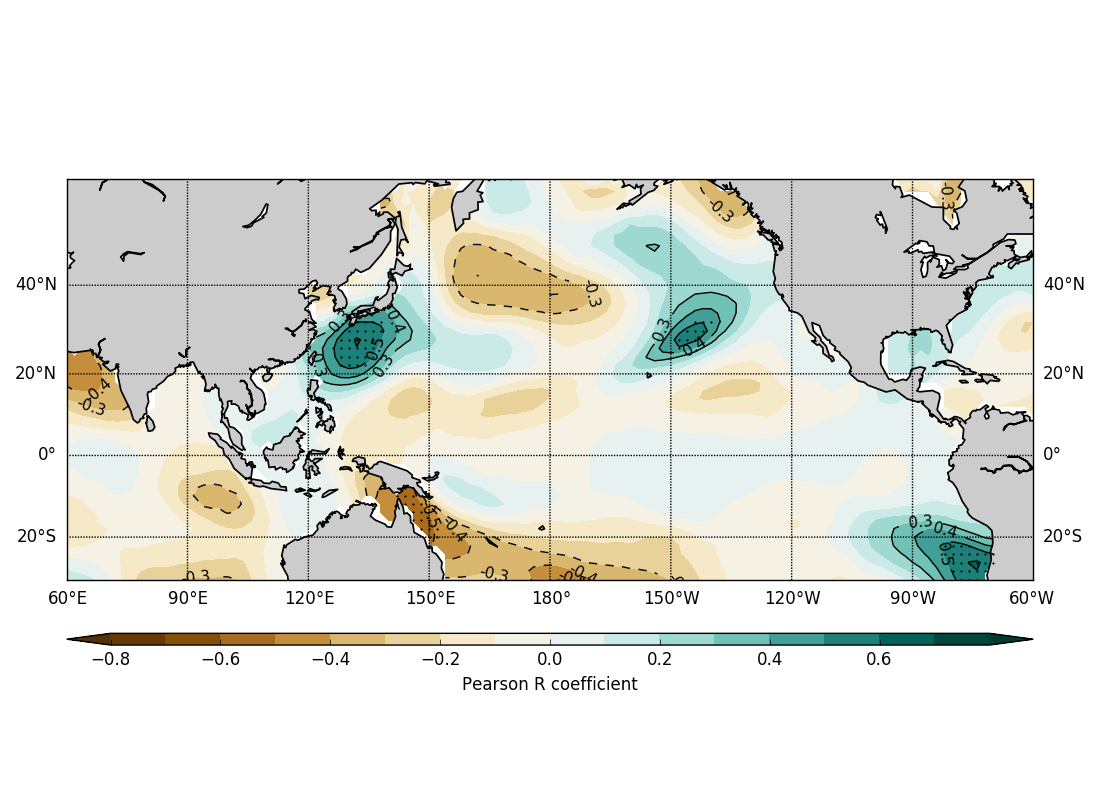
\includegraphics[width=1.8in]{sst_prev_JFM&countJJASO63inp_intcorr_late.png}}
	
	\subfloat[2a]{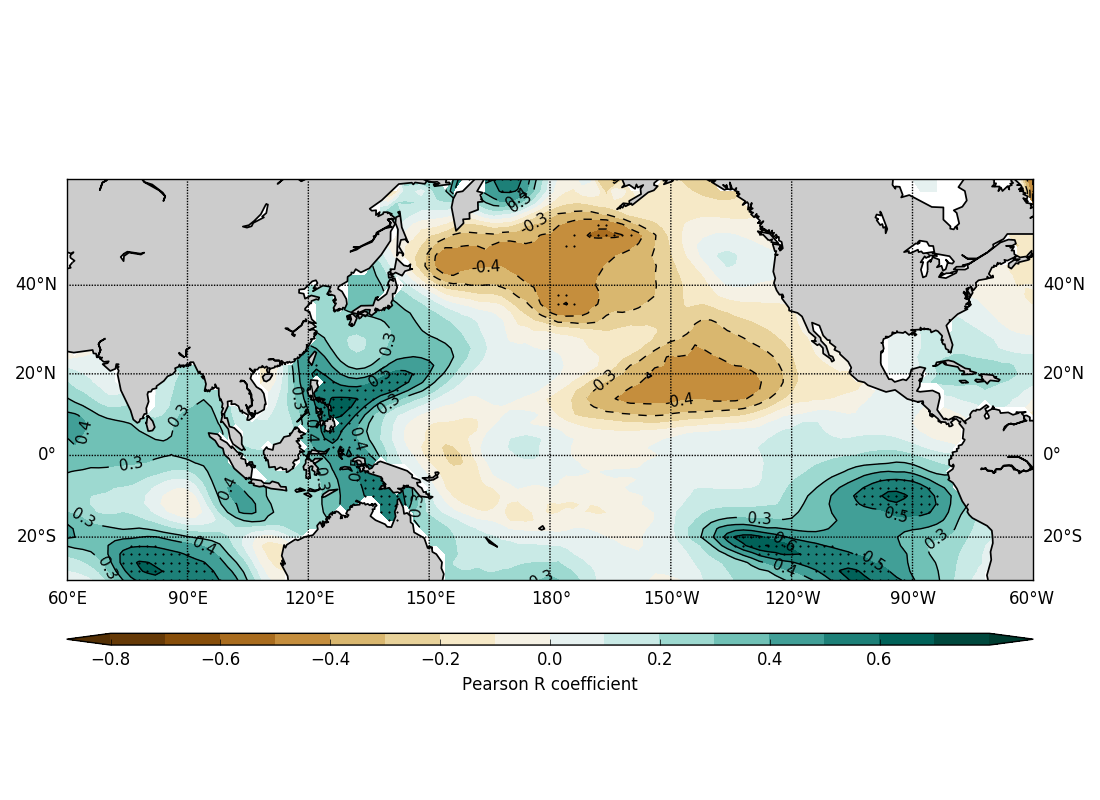
\includegraphics[width=1.8in]{sst_prev_JFM&countJJASO95inp_intcorr_early.png}}
	\subfloat[2a]{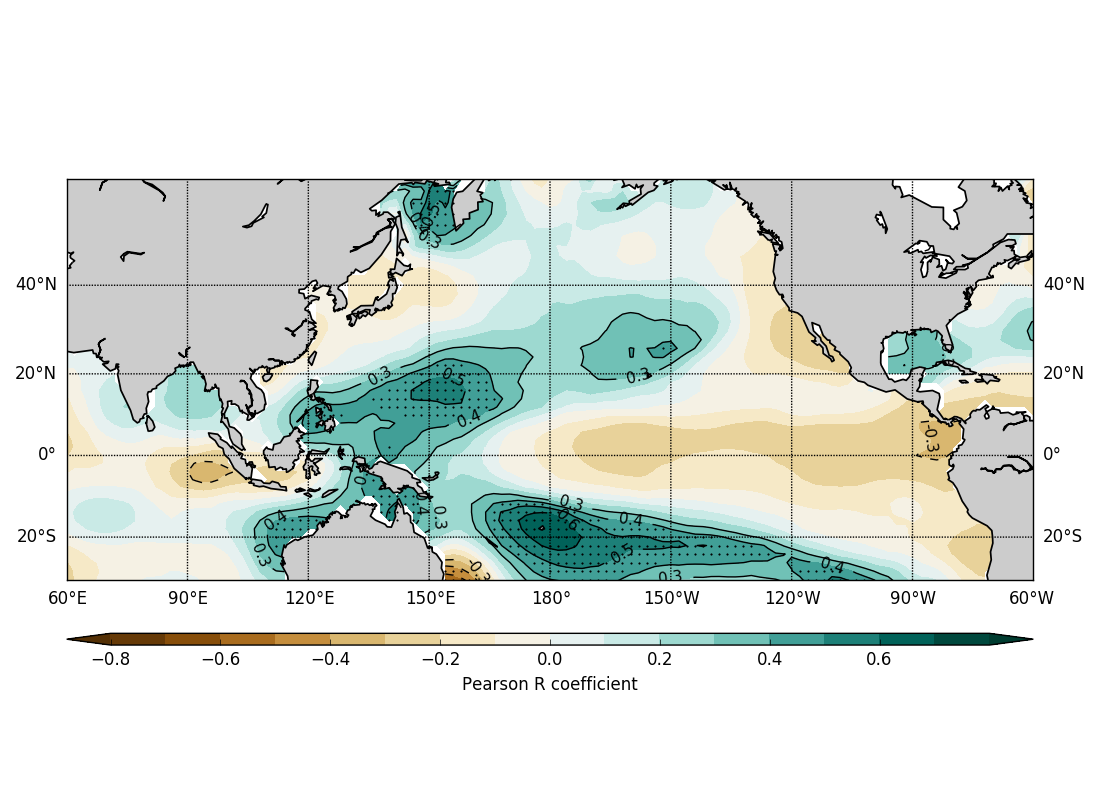
\includegraphics[width=1.8in]{sst_prev_JFM&countJJASO95inp_intcorr_mid.png}}
	\subfloat[2a]{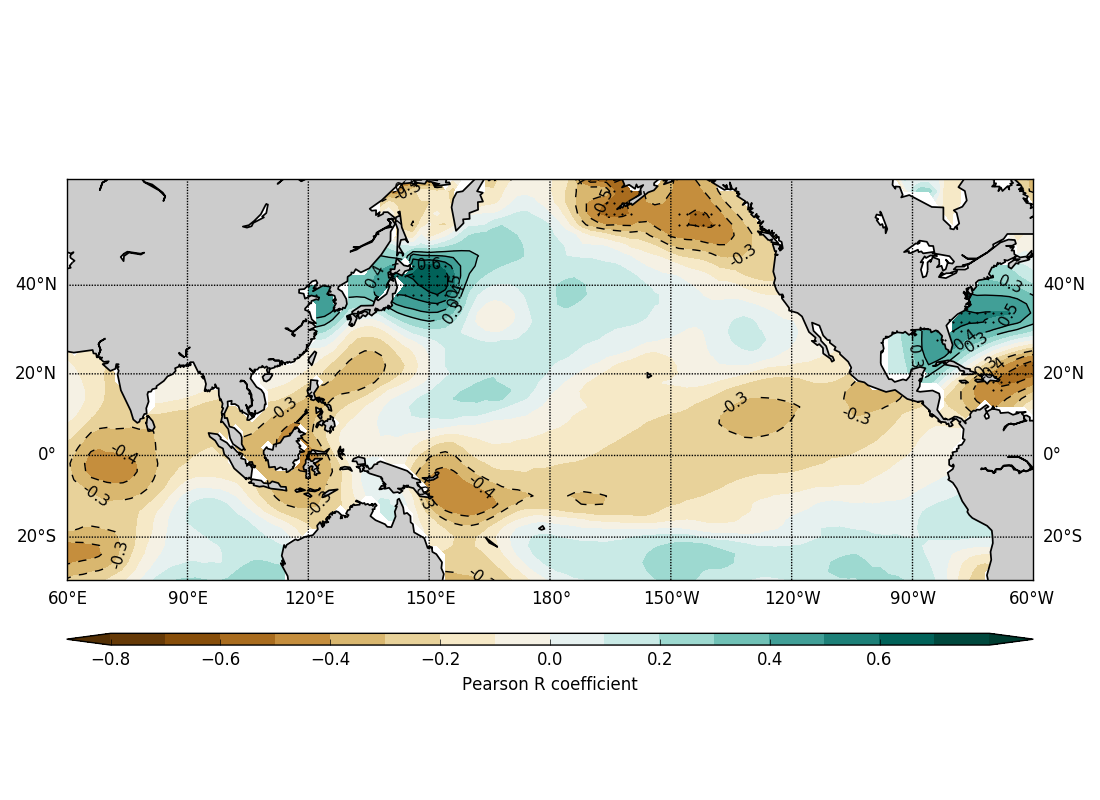
\includegraphics[width=1.8in]{sst_prev_JFM&countJJASO95inp_intcorr_late.png}}
	
	\subfloat[2a]{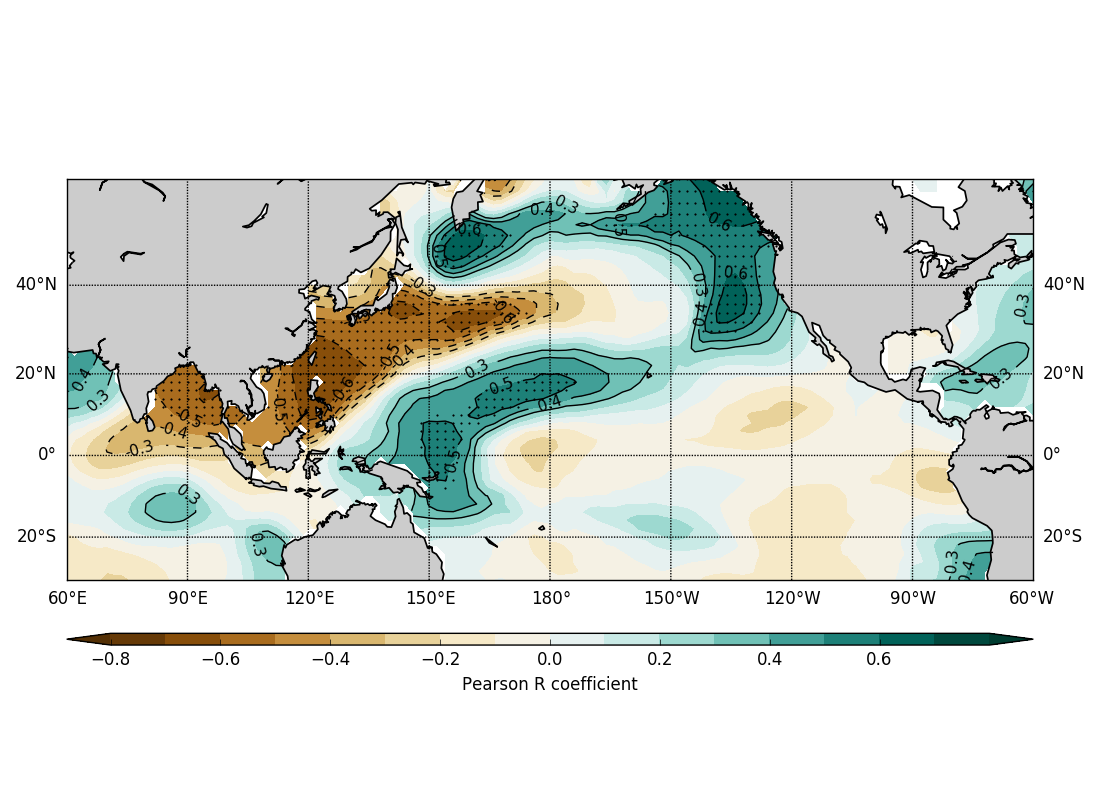
\includegraphics[width=1.8in]{sst_prev_JFM&countJJASOplusinp_intcorr_early.png}}
	\subfloat[2a]{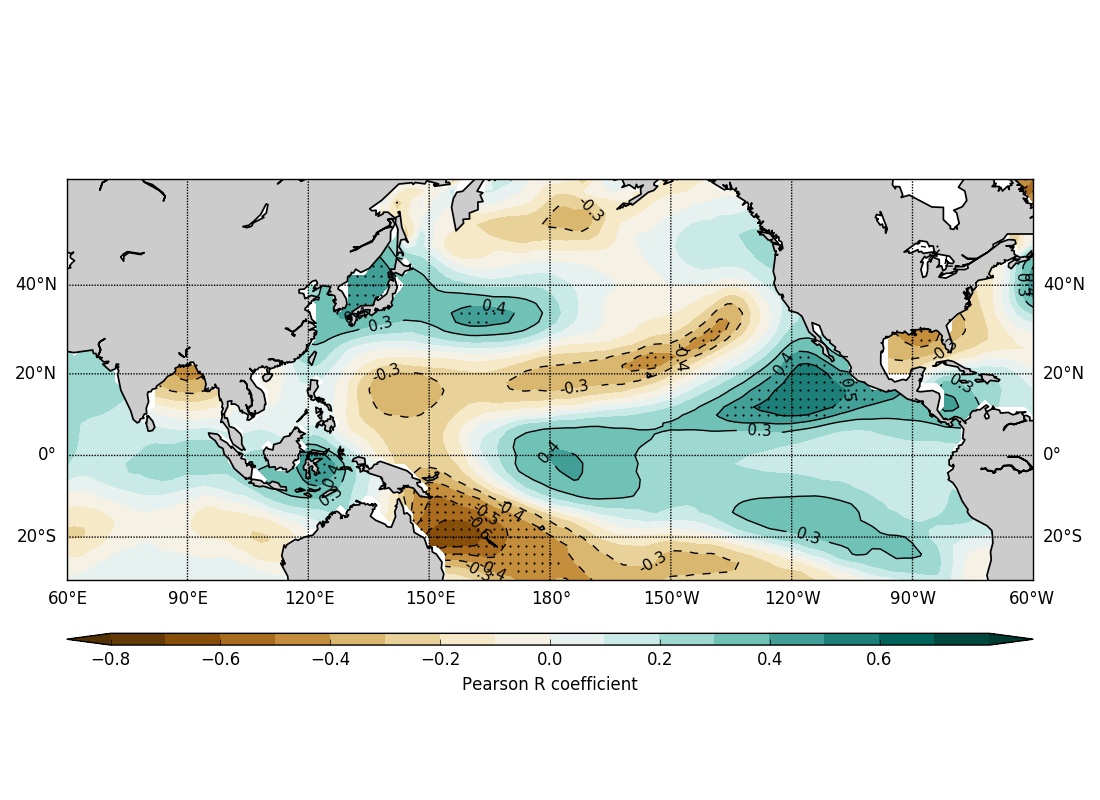
\includegraphics[width=1.8in]{sst_prev_JFM&countJJASOplusinp_intcorr_mid.png}}
	\subfloat[2a]{\includegraphics[width=1.8in]{sst_prev_JFM&countJJASOplusinp_intcorr_late.png}}
	\caption{SST-JFM-1 correlated with count-JJASO for within the domain for 1958-1975 (1), 1976-1997 (2), 1998-2014 (3). a. Tropical storms and tropical depressions. b. Categories 1,2 c. Categories 3, 4, 5.  Stippling shows grid points with significant correlation at 95th percentile} \label{fig:corr_prevJFM_periods} 
\end{figure} 

Figure \ref{fig:corr_prevJFM_periods} shows the correlation maps between count-JJASO and SST-JFM-1 broken down into three different periods for the three categories. 
The strong positive correlation off the east coast of China and into the Bay of Bengal is dominated by the early period (cold PDO), for both the weak storms (1a) and intense storms (1c). For the weak storms, the negative correlation to the east of this region at 10-20N remains, although the positive signal is not apparent. During the mixed phase, there is a region of signficant positive correlation in the East China Sea, although this is slightly weaker than the mean over the period and no signal in the Bay of Bengal.
For the strong storms, during the warm period and mixed period, there are no significant correlations in the region of interest, although in the mixed period, the opposing correlation to the east of the region is shown.



It is not only the sea surface that affects tropical storm activity, but the deeper ocean can have an influence (ref section). Therefore the ocean heat content (OHC) (to 100m?) is also investigated.

\begin{figure} % remove [h] and this appeared in the correct place
	\centering % Y:/Code_Data/Chapter1/Plots_new/Charts/
	\noindent\includegraphics[width=30pc,angle=0]{ohc_JJASO_mean.png}
	%	\noindent\includegraphics[width=30pc,angle=0]{Y:/Code_Data/Chapter1/Plots_new/Charts/ohc_JJASO_std.png}\\
	\caption{OHC (to 100 m) mean during JJASO}\label{fig:OHC_JJASO}
\end{figure}

The mean OHC to 100m during the JJASO season shows a very similar pattern to SST (figure \ref{fig:OHC_JJASO}), with an area of relatively warm water extending from the tropics to approximately 30N. Water in the west of the basin is warmer than the east, where there is upwelling of cooler water.


Figure \ref{fig:ohc_currJJASO} shows the correlations with OHC-JJASO and count-JJASO.

\begin{figure}
	\centering % Y:/Code_Data/Chapter1/Plots_new/Corr_maps_final/count/inp_int/ohc/

	\subfloat[2a]{\includegraphics[width=2.6in]{ohc_curr_JJASO&countJJASO63inp_intcorr_total.png}}
%	\subfloat[2a]{\includegraphics[width=2.6in]{Y:/Code_Data/Chapter1/Plots_new/Corr_maps_final/count/inp_int/ohc/ohc_curr_JJASO&countJJASO95inp_intcorr_total.png}}
	\subfloat[2a]{\includegraphics[width=2.6in]{ohc_curr_JJASO&countJJASOplusinp_intcorr_total.png}}
%	\subfloat[2a]{\includegraphics[width=2.6in]{Y:/Code_Data/Chapter1/Plots_new/Corr_maps_final/count/inp_int/ohc/ohc_curr_JJASO&countJJASOallcatsinp_intcorr_total.png}}
	\caption{OHC-JJASO correlated with count-JJASO for within the domain over the training period 1958-2007. a. Tropical storms and tropical depressions. b. Categories 1,2 c. Categories 3, 4, 5. Stippling shows grid points with significant correlation at 95th percentile} \label{fig:ohc_currJJASO} 
\end{figure} 

Ocean heat content (OHC) (to 100 m) was also analysed in the same method as above. Data is at twice the resolution of SST (1 rather than 2 degrees) and so more detail in spatial patterns is apparent. 
The positive correlations in the Philippines Sea, East China Sea and along the Kuroshio current are not as clear in OHC as with SST, although there are some stippled grid points, especially close to the east coast of the mainland.

%Correlation maps show a very similar relationship with ACE and frequency as the SST (figure \ref{fig:corr_JJASO}), although are at twice the resolution. During the storm season, the OHC show some significant negative correlation in the eastern equatorial Pacific, not present in the SST maps, and does not show the positive significant areas off the east coast of Asia and in the vicinity of Japan. 

The positive correlation in the northern Pacific is present in SST and OHC (figures) for the intense storms, with a more strongly negative correlation below this.

OHC-JFM-1 shows the opposing correlations for weak and intense storms in the East China Sea, although this is less extensive and does not extend into the Bay of Bengal and towards the Aleutian Islands.

\begin{figure}
	\centering
	% Y:/Code_Data/Chapter1/Plots_new/Corr_maps_final/count/inp_int/ohc/
	\subfloat[2a]{\includegraphics[width=2.6in]{ohc_prev_JFM&countJJASO63inp_intcorr_total.png}}

	\subfloat[2a]{\includegraphics[width=2.6in]{ohc_prev_JFM&countJJASOplusinp_intcorr_total.png}}

	\caption{OHC-JFM-1 correlated with count-JJASO for within the domain over the training period 1958-2007. a. Tropical storms and tropical depressions. b. Categories 1,2 c. Categories 3, 4, 5. Stippling shows grid points with significant correlation at 95th percentile} \label{fig:ohc_prevJFM} 
\end{figure} 

As well as these oceanic variables, a number of atmospheric variables were analysed using the JRA-55 reanalysis data.
% Examine if there is an atmospheric pattern related to the ACE or count in JJASO. Same correlation plots, but with mslp, geopotential height, ]
%With mslp and geopotential check out monsoon trough, subtropical high

\subsubsection{Atmospheric variables}

The ocean and atmosphere interact through the marine boundary layer (MBL) and likely that signals are...

\begin{figure}
	\centering
	%	\subfloat[1a]{\includegraphics[width=2.4in]{Y:/Code_Data/Chapter1/Plots_new/Corr_maps/ACE/inpoly/curr_sst_JJASO&ACEJJASO63inpolycorr_trainmslp.png}}  % Y:/Code_Data/Chapter1/Plots_new/Corr_maps_final/count/inp_int/mslp/
	\subfloat[2a]{\includegraphics[width=2.6in]{mslp_curr_JJASO&countJJASO63inp_intcorr_total.png}}
	\subfloat[2a]{\includegraphics[width=2.6in]{geop_curr_JJASO&countJJASO63inp_intcorr_total.png}}
	%\subfloat[1b]{\includegraphics[width=2.4in]{Y:/Code_Data/Chapter1/Plots_new/Corr_maps/ACE/inpoly/curr_sst_JJASO&ACEJJASO95inpolycorr_trainmslp.png}}
%	\subfloat[2a]{\includegraphics[width=2.6in]{Y:/Code_Data/Chapter1/Plots_new/Corr_maps_final/count/inp_int/mslp/mslp_curr_JJASO&countJJASO95inp_intcorr_total.png}}
%	\subfloat[2a]{\includegraphics[width=2.6in]{Y:/Code_Data/Chapter1/Plots_new/Corr_maps_final/count/inp_int/geop/geop_curr_JJASO&countJJASO95inp_intcorr_total.png}}
	%\subfloat[1c]{\includegraphics[width=2.4in]{Y:/Code_Data/Chapter1/Plots_new/Corr_maps/ACE/inpoly/curr_sst_JJASO&ACEJJASOplusinpolycorr_trainmslp.png}}
	\subfloat[2a]{\includegraphics[width=2.6in]{mslp_curr_JJASO&countJJASOplusinp_intcorr_total.png}}
	\subfloat[2a]{\includegraphics[width=2.6in]{geop_curr_JJASO&countJJASOplusinp_intcorr_total.png}}
	
%	\subfloat[2a]{\includegraphics[width=2.6in]{Y:/Code_Data/Chapter1/Plots_new/Corr_maps_final/count/inp_int/mslp/mslp_curr_JJASO&countJJASOallcatsinp_intcorr_total.png}}
%	\subfloat[2d]{\includegraphics[width=2.4in]{Y:/Code_Data/Chapter1/Plots_new/Corr_maps/count/inp_int/curr_sst_JJASO&countJJASOallcatsinp_intcorr_traingeop.png}}	
	\caption{MSLP-JJASO and geop500-JJASO correlated with count-JJASO for within the domain over the training period 1958-2007. a. Tropical storms and tropical depressions. b. Categories 1,2 c. Categories 3, 4, 5. Stippling shows grid points with significant correlation at 95th percentile} \label{fig:corr_curr_JJASO_mslpgeop} 
\end{figure} 

%\begin{figure}
%	\centering
%	%	\subfloat[1a]{\includegraphics[width=2.4in]{Y:/Code_Data/Chapter1/Plots_new/Corr_maps/ACE/inpoly/curr_sst_JJASO&ACEJJASO63inpolycorr_trainmslp.png}} 
%	\subfloat[2a]{\includegraphics[width=2.4in]{Y:/Code_Data/Chapter1/Plots_new/Corr_maps/count/inp_int/curr_sst_JJASO&countJJASO63inp_intcorr_traingeop.png}}
%	%\subfloat[1b]{\includegraphics[width=2.4in]{Y:/Code_Data/Chapter1/Plots_new/Corr_maps/ACE/inpoly/curr_sst_JJASO&ACEJJASO95inpolycorr_trainmslp.png}}
%	\subfloat[2b]{\includegraphics[width=2.4in]{Y:/Code_Data/Chapter1/Plots_new/Corr_maps/count/inp_int/curr_sst_JJASO&countJJASO95inp_intcorr_traingeop.png}}
%	%\subfloat[1c]{\includegraphics[width=2.4in]{Y:/Code_Data/Chapter1/Plots_new/Corr_maps/ACE/inpoly/curr_sst_JJASO&ACEJJASOplusinpolycorr_trainmslp.png}}
%	\subfloat[2c]{\includegraphics[width=2.4in]{Y:/Code_Data/Chapter1/Plots_new/Corr_maps/count/inp_int/curr_sst_JJASO&countJJASOplusinp_intcorr_traingeop.png}}
%	\caption{geopotential(500)-JJASO correlated with count-JJASO for within the domain over the training period 1958-2007. a. Tropical storms and tropical depressions. b. Categories 1,2 c. Categories 3, 4, 5. Stippling shows grid points with significant correlation at 95th percentile} \label{fig:corr_curr_JJASO_geop} 
%\end{figure} 
Tie these atm results into sst results

Mean sea level pressure (mslp) and 500 hPa geopotential height are correlated with count-JJASO (figure \ref{fig:corr_curr_JJASO_mslpgeop}). The patterns are almost identical.

For the low intensity storms, there is an area of significant correlation in the East China Sea and South China Sea, which is at the same location as the significant positive SST signal. When mslp is anomalously high (and SST anomalously low), there is a decrease in the frequency of low intensity storms making landfall in the domain. There is a positive correlation with mslp in parts of Alaska and the northeast coast of the USA.
For the high intensity storms, there is a region of signficant positive correlation in the northern North Pacific, although this is shifted to the north and is weaker and smaller.


Figure \ref{fig:mslp_JJASO} shows the mean mslp during JJASO, and the subtropical high is clearly visible, centred off the west coast of the USA and extending westwards towards Asia. The mslp during JJASO / all year? across the mid and high latitudes is more variable year to year than across the Tropics.

\begin{figure} % remove [h] and this appeared in the correct place
 % Y:/Code_Data/Chapter1/Plots_new/Charts/
	\subfloat[a]{\includegraphics[width=3.5in]{mslp_JJASO_mean.png}} 
	\subfloat[b]{\includegraphics[width=3.5in]{mslp_JJASO_std.png}} 
	\subfloat[c]{\includegraphics[width=3.5in]{mslp_JFM_mean.png}} 
	\subfloat[d]{\includegraphics[width=3.5in]{mslp_JFM_std.png}} 
	
	\caption{MSLP climatology (a) mean and (b) standard deviation during the JJASO season}\label{fig:mslp_JJASO}
\end{figure}


In JFM-1, there are no strong correlations over the region of SST. However, there are opposing correlations running north to south down China, although only significant for the intense storms. There are large regions of positive SST over the ocean for the weak storms, notably in the Indian Ocean.


\begin{figure}
	\centering
%	\subfloat[2a]{\includegraphics[width=2.6in]{Y:/Code_Data/Chapter1/Plots_new/Corr_maps_final/ACE/inpoly/mslp/mslp_prev_JFM&ACEJJASO63inpolycorr_total.png}}
	\subfloat[2a]{\includegraphics[width=2.6in]{Y:/Code_Data/Chapter1/Plots_new/Corr_maps_final/count/inp_int/mslp/mslp_prev_JFM&countJJASO63inp_intcorr_total.png}}
%	\subfloat[2a]{\includegraphics[width=2.6in]{Y:/Code_Data/Chapter1/Plots_new/Corr_maps_final/ACE/inpoly/mslp/mslp_prev_JFM&ACEJJASO95inpolycorr_total.png}}
%	\subfloat[2a]{\includegraphics[width=2.6in]{Y:/Code_Data/Chapter1/Plots_new/Corr_maps_final/count/inp_int/mslp/mslp_prev_JFM&countJJASO95inp_intcorr_total.png}}
%	\subfloat[2a]{\includegraphics[width=2.6in]{Y:/Code_Data/Chapter1/Plots_new/Corr_maps_final/ACE/inpoly/mslp/mslp_prev_JFM&ACEJJASOplusinpolycorr_total.png}}
	\subfloat[2a]{\includegraphics[width=2.6in]{Y:/Code_Data/Chapter1/Plots_new/Corr_maps_final/count/inp_int/mslp/mslp_prev_JFM&countJJASOplusinp_intcorr_total.png}}
%	\subfloat[2a]{\includegraphics[width=2.6in]{Y:/Code_Data/Chapter1/Plots_new/Corr_maps_final/ACE/inpoly/mslp/mslp_prev_JFM&ACEJJASOallcatsinpolycorr_total.png}}
%	\subfloat[2a]{\includegraphics[width=2.6in]{Y:/Code_Data/Chapter1/Plots_new/Corr_maps_final/count/inp_int/mslp/mslp_prev_JFM&countJJASOallcatsinp_intcorr_total.png}}
	
	\caption{MSLP-JFM-1 correlated with count-JJASO for within the domain over the training period 1958-2007. a. Tropical storms and tropical depressions. b. Categories 1,2 c. Categories 3, 4, 5. Stippling shows grid points with significant correlation at 95th percentile} \label{fig:corr_prevJFM_mslp} 
\end{figure} 

Geopotential height is good for the mid-latitudes. In the Tropics, pressure fields and geopotential are flat because of a weak Coriolis. Look at winds in Tropics. Because not constrained by geostrophy in Tropics.

The zonal wind has an opposing relationship with frequency between low and high in a region upstream of landfall.
The winds are examined at 500 hPa and 850 hPa. 
During JJASO, there is no strong correlation where the SST signal was in the Philippine Sea and East China Sea, but there is a significant negative correlation along the Kuroshio, where a correlation was seen in the weak storms. Relate to SST anomaly. Also for the weak storms, an area approximately 20 degrees (2000 km) to the east of landfall is significant positive correlation. When there is anomalous westerly winds (or reduced easterlies), there is an increased frequency of weak storms. In a similar location, to the east of the landfall domain, there is a negative correlation for the intense storms. When the wind is anomalously easterly (ie reduced u wind), there is an increased frequency of intense storms making landfall in the region.


\begin{figure}
	\centering
	\subfloat[2a]{\includegraphics[width=2.6in]{Y:/Code_Data/Chapter1/Plots_new/Corr_maps_final/count/inp_int/u500/u500_curr_JJASO&countJJASO63inp_intcorr_total.png}}
	\subfloat[2a]{\includegraphics[width=2.6in]{Y:/Code_Data/Chapter1/Plots_new/Corr_maps_final/count/inp_int/u850/u850_curr_JJASO&countJJASO63inp_intcorr_total.png}}		%\subfloat[2a]{\includegraphics[width=2.6in]{Y:/Code_Data/Chapter1/Plots_new/Corr_maps_final/count/inp_int/u500/u500_curr_JJASO&countJJASO95inp_intcorr_total.png}}
	%\subfloat[2b]{\includegraphics[width=2.4in]{Y:/Code_Data/Chapter1/Plots_new/Corr_maps/count/inp_int/curr_sst_JJASO&countJJASO95inp_intcorr_trainu850.png}}		\subfloat[2a]{\includegraphics[width=2.6in]{Y:/Code_Data/Chapter1/Plots_new/Corr_maps_final/count/inp_int/u500/u500_curr_JJASO&countJJASOplusinp_intcorr_total.png}}
	\subfloat[2a]{\includegraphics[width=2.6in]{Y:/Code_Data/Chapter1/Plots_new/Corr_maps_final/count/inp_int/u500/u500_curr_JJASO&countJJASOplusinp_intcorr_total.png}}
	\subfloat[2a]{\includegraphics[width=2.6in]{Y:/Code_Data/Chapter1/Plots_new/Corr_maps_final/count/inp_int/u850/u850_curr_JJASO&countJJASOplusinp_intcorr_total.png}}
%	\subfloat[2a]{\includegraphics[width=2.6in]{Y:/Code_Data/Chapter1/Plots_new/Corr_maps_final/count/inp_int/u500/u500_curr_JJASO&countJJASOallcatsinp_intcorr_total.png}}
%	\subfloat[2c]{\includegraphics[width=2.4in]{Y:/Code_Data/Chapter1/Plots_new/Corr_maps/count/inp_int/curr_sst_JJASO&countJJASOallcatsinp_intcorr_trainu850.png}}

	\caption{u-JJASO correlated with count-JJASO for within the domain over the training period 1958-2007.(1) u500, (2) u850. a. Tropical storms and tropical depressions. b. Categories 1,2 c. Categories 3, 4, 5. Stippling shows grid points with significant correlation at 95th percentile} \label{fig:corr_curr_JJASO_u} 
\end{figure} 





\begin{figure}
	\centering
	\subfloat[2a]{\includegraphics[width=2.6in]{Y:/Code_Data/Chapter1/Plots_new/Corr_maps_final/count/inp_int/u500/u500_prev_JFM&countJJASO63inp_intcorr_total.png}}
	\subfloat[2a]{\includegraphics[width=2.6in]{Y:/Code_Data/Chapter1/Plots_new/Corr_maps_final/count/inp_int/u850/u850_prev_JFM&countJJASO63inp_intcorr_total.png}}	%\subfloat[2a]{\includegraphics[width=2.6in]{Y:/Code_Data/Chapter1/Plots_new/Corr_maps_final/count/inp_int/u500/u500_prev_JFM&countJJASO95inp_intcorr_total.png}}
%	\subfloat[2b]{\includegraphics[width=2.4in]{Y:/Code_Data/Chapter1/Plots_new/Corr_maps/count/inp_int/prev_sst_JFM&countJJASO95inp_intcorr_trainu850.png}}		\subfloat[2a]{\includegraphics[width=2.6in]{Y:/Code_Data/Chapter1/Plots_new/Corr_maps_final/count/inp_int/u500/u500_prev_JFM&countJJASOplusinp_intcorr_total.png}}
	\subfloat[2a]{\includegraphics[width=2.6in]{Y:/Code_Data/Chapter1/Plots_new/Corr_maps_final/count/inp_int/u500/u500_prev_JFM&countJJASOplusinp_intcorr_total.png}}		\subfloat[2a]{\includegraphics[width=2.6in]{Y:/Code_Data/Chapter1/Plots_new/Corr_maps_final/count/inp_int/u850/u850_prev_JFM&countJJASOplusinp_intcorr_total.png}}
%	\subfloat[2a]{\includegraphics[width=2.6in]{Y:/Code_Data/Chapter1/Plots_new/Corr_maps_final/count/inp_int/u500/u500_prev_JFM&countJJASOallcatsinp_intcorr_total.png}}
%	\subfloat[2c]{\includegraphics[width=2.4in]{Y:/Code_Data/Chapter1/Plots_new/Corr_maps/count/inp_int/prev_sst_JFM&countJJASOallcatsinp_intcorr_trainu850.png}}
	\caption{u-JFM-1 correlated with count-JJASO for within the domain over the training period 1958-2007.(1) u500, (2) u850. a. Tropical storms and tropical depressions. b. Categories 1,2 c. Categories 3, 4, 5. Stippling shows grid points with significant correlation at 95th percentile} \label{fig:corr_prevJFM_u} 
\end{figure} 

Temp JJASO shows same SST patterns with nothing interesting over land. No need to show it.

%\begin{figure}
%	\centering
%	\subfloat[2a]{\includegraphics[width=2.6in]{Y:/Code_Data/Chapter1/Plots_new/Corr_maps_final/count/inp_int/temp1000/temp1000_curr_JJASO&countJJASO63inp_intcorr_total.png}}
%	\subfloat[2a]{\includegraphics[width=2.6in]{Y:/Code_Data/Chapter1/Plots_new/Corr_maps_final/count/inp_int/temp850/temp850_curr_JJASO&countJJASO63inp_intcorr_total.png}}	
%	\subfloat[2a]{\includegraphics[width=2.6in]{Y:/Code_Data/Chapter1/Plots_new/Corr_maps_final/count/inp_int/temp1000/temp1000_curr_JJASO&countJJASOplusinp_intcorr_total.png}}
%	\subfloat[2a]{\includegraphics[width=2.6in]{Y:/Code_Data/Chapter1/Plots_new/Corr_maps_final/count/inp_int/temp850/temp850_curr_JJASO&countJJASOplusinp_intcorr_total.png}}	
%	\caption{Temp1000-JJASO correlated with count-JJASO for within the domain over the training period 1958-2007. a. Tropical storms and tropical depressions. b. Categories 1,2 c. Categories 3, 4, 5. Stippling shows grid points with significant correlation at 95th percentile} \label{fig:corr_JJASO_temp} 
%\end{figure} 

Temperature at 1000 hPa shows the same opposing significant relationships for the weak and intense storms in the South China Sea as seen with SST. This field gives additional information over land and also shows that this relationship extends onto land a couple of hundred kilometres. Point of showing temp is that anomaly extends onto land.

\begin{figure}
	\centering
	\subfloat[2a]{\includegraphics[width=2.6in]{Y:/Code_Data/Chapter1/Plots_new/Corr_maps_final/count/inp_int/temp1000/temp1000_prev_JFM&countJJASO63inp_intcorr_total.png}}
	\subfloat[2a]{\includegraphics[width=2.6in]{Y:/Code_Data/Chapter1/Plots_new/Corr_maps_final/count/inp_int/temp850/temp850_prev_JFM&countJJASO63inp_intcorr_total.png}}	%\subfloat[2a]{\includegraphics[width=2.6in]{Y:/Code_Data/Chapter1/Plots_new/Corr_maps_final/count/inp_int/temp1000/temp1000_prev_JFM&countJJASO95inp_intcorr_total.png}}
	%\subfloat[2a]{\includegraphics[width=2.6in]{Y:/Code_Data/Chapter1/Plots_new/Corr_maps_final/count/inp_int/temp850/temp850_prev_JFM&countJJASO95inp_intcorr_total.png}}
	\subfloat[2a]{\includegraphics[width=2.6in]{Y:/Code_Data/Chapter1/Plots_new/Corr_maps_final/count/inp_int/temp1000/temp1000_prev_JFM&countJJASOplusinp_intcorr_total.png}}
	\subfloat[2a]{\includegraphics[width=2.6in]{Y:/Code_Data/Chapter1/Plots_new/Corr_maps_final/count/inp_int/temp850/temp850_prev_JFM&countJJASOplusinp_intcorr_total.png}}	%\subfloat[2a]{\includegraphics[width=2.6in]{Y:/Code_Data/Chapter1/Plots_new/Corr_maps_final/count/inp_int/temp1000/temp1000_prev_JFM&countJJASOallcatsinp_intcorr_total.png}}
	%\subfloat[2a]{\includegraphics[width=2.6in]{Y:/Code_Data/Chapter1/Plots_new/Corr_maps_final/count/inp_int/temp850/temp850_prev_JFM&countJJASOallcatsinp_intcorr_total.png}}
	\caption{Temp1000-JFM-1 correlated with count-JJASO for within the domain over the training period 1958-2007. a. Tropical storms and tropical depressions. b. Categories 1,2 c. Categories 3, 4, 5. Stippling shows grid points with significant correlation at 95th percentile} \label{fig:corr_prevJFM_temp} 
\end{figure} 


Ocean forcing the atmosphere vs atmosphere forcing ocean.


In order to examine the cause of these SST anomalies off the east coast, sensible and latent heat flux are examined.
JFM plots - save year, do I see re-emergence? yes!

SST anomalies in winter because driven by atmospheric systems (active). Summer has a shallow mixed layer. Anomalies stay deep. Next winter, mixed up - re-emergence.

\subsubsection{Heat flux}

Heat flux W per m\textsuperscript{2}
Latent heat flux is the flux of heat from the Earth's surface to the atmosphere that is associated with evaporation of water at the surface and subsequent condensation of water vapor in the troposphere. 
From Arnaud 1998 paper
Lag covariance between surface heat flux and SST anomalies, we have shown that the turbulent heat
flux plays a dual forcing and damping role. As discussed in Frankignoul (1985), the heat flux
feedback is dominated by the turbulent heat fluxes (latent and sensible heat flux), and it can be estimated from
the response of atmospheric general circulation models (AGCMs) to prescribed SST anomalies. However, the
relationship between the SST and heat flux anomaly fields may be rather complex and seems model dependent
and, in some cases, a function of the location and polarity the SST anomaly
LHF plots in prev year - lots of significant spots, but moves around each month

\begin{figure}[h]
	\centering
	\noindent\includegraphics[width=26pc,angle=0]{H:/Documents/Thesis/phd-thesis-template-2.2.2_AC/phd-thesis-template-2.2.2/Figs/heat_flux_pic.png}
	\caption{Need to sort out this diagram}\label{fig:heat_flux}
\end{figure}



\begin{figure} % remove [h] and this appeared in the correct place
	
	\subfloat[a]{\includegraphics[width=3.5in]{Y:/Code_Data/Chapter1/Plots_new/Charts/hf_JJASO_mean.png}} 
	\subfloat[b]{\includegraphics[width=3.5in]{Y:/Code_Data/Chapter1/Plots_new/Charts/hf_JJASO_std.png}} 
	\subfloat[c]{\includegraphics[width=3.5in]{Y:/Code_Data/Chapter1/Plots_new/Charts/hf_JFM_mean.png}} 
	\subfloat[d]{\includegraphics[width=3.5in]{Y:/Code_Data/Chapter1/Plots_new/Charts/hf_JFM_std.png}} 
	
	\caption{Heat flux climatology (a) mean and (b) standard deviation during the JJASO season}\label{fig:HF_climat}
\end{figure}


During the JJASO season, mean heat flux (latent plus sensible) is generally consistent across longitude bands, with lower values towards the poles. In the winter (JFM), the largest heat fluxes are dominated in a small region around the Kuroshio current. Which is ... This warm ocean current transfers heat upwards into the relatively cool atmosphere.
Tropics - ocean current create sst anomalies, e.g. El Nino.

Latent heat flux is what percentage of sensible?

A note about standard deviation. Do not need to show plot.



\begin{figure}
	\centering
	\subfloat[2a]{\includegraphics[width=2.6in]{Y:/Code_Data/Chapter1/Plots_new/Corr_maps_final/count/inp_int/hf/hf_curr_JJASO&countJJASO63inp_intcorr_total.png}}
	\subfloat[2a]{\includegraphics[width=2.6in]{Y:/Code_Data/Chapter1/Plots_new/Corr_maps_final/count/inp_int/hf/hf_curr_JJASO&countJJASOplusinp_intcorr_total.png}}

	\caption{HF-JJASO and count } \label{fig:corr_JJASO_hf} 
\end{figure} 

Heat flux during JJASO and the plus count has the same positive correlation in the northern North Pacific. However, the positive correlation seen with SST for the weak storms in the Philippine Sea, East China Sea is not present.

\begin{figure}
	\centering
	\subfloat[2a]{\includegraphics[width=2.6in]{Y:/Code_Data/Chapter1/Plots_new/Corr_maps_final/count/inp_int/hf/hf_prev_JFM&countJJASO63inp_intcorr_total.png}}
	\subfloat[2a]{\includegraphics[width=2.6in]{Y:/Code_Data/Chapter1/Plots_new/Corr_maps_final/count/inp_int/hf/hf_prev_JFM&countJJASOplusinp_intcorr_total.png}}
	
	\caption{HF JFM-1 and count } \label{fig:corr_JFN-1_hf} 
\end{figure} 

The signals in the Bay of Bengal and off the east coast of China in JFM-1 seen with SST is not apparent when examining heat flux.
%\begin{figure}
%	\centering
%	\subfloat[2a]{\includegraphics[width=2.4in]{Y:/Code_Data/Chapter1/Plots_new/Corr_maps_detrend/hf_sst/hfJune_SSTJune_49y.png}}
%	\subfloat[2a]{\includegraphics[width=2.4in]{Y:/Code_Data/Chapter1/Plots_new/Corr_maps_detrend/hf_sst/hfJuly_SSTJuly_49y.png}}
%	\subfloat[2a]{\includegraphics[width=2.4in]{Y:/Code_Data/Chapter1/Plots_new/Corr_maps_detrend/hf_sst/hfAug_SSTAug_49y.png}}	
%	\subfloat[2a]{\includegraphics[width=2.4in]{Y:/Code_Data/Chapter1/Plots_new/Corr_maps_detrend/hf_sst/hfSept_SSTSept_49y.png}}
%	\subfloat[2a]{\includegraphics[width=2.4in]{Y:/Code_Data/Chapter1/Plots_new/Corr_maps_detrend/hf_sst/hfOct_SSTOct_49y.png}}
%	
%	\caption{SST HF correlation for different months across the 49 years} \label{fig:corr_sst_hf} 
%\end{figure} 
% Need to stipple, remove colourts around 0-0.2. Put on same scale.
These plots compare the time series across 49 or 48? years of a specific month hf and sst.
Only match at every 10 degrees, i.e. 0, 10, 20 lat and lon. Contour has smoothed lines, so concentrate on where point is significant.

Present in all JJASO months is a positive correlation between surface heat flux and SST in the El Nino region (region 3.4?). During years when the hf or sst is anomalously increased during the month, the hf or sst is also increased. Is it significant?

Focus on key areas where see anomalies in JJASO (fig 2.4). - EJAP, SCS, BOB, NNPac
Which month has the strongest correlations?

Select only which plots are of interest - how hf relates to sst in monthly lags.
ADD JFM
Analyse August or June???? as in the middle of JJASO. then mention how the plots look different depending on the starting month.

Figure \ref{fig:corr_sstJan_hflag} shows the spatial correlations between January SST and heat flux from November, December, January, February and March, with stipples at p less than 0.05. The maps show interpolated fields as values are only available every 10 degrees longitude and latitude. The positive correlation in the equatorial region is apparent in all plots, however, weakens and is more central rather than east as the heat flux months progress. The correlation with December heat flux shows negative correlation, significant over most of north of 20N. This correlation is weaker and less coherent using November and January heat flux, and in February and March, is generally positive although only significant in places. North of 20N, the December heat flux is negatively correlated with January SST as  

\begin{figure}
	\centering
	\subfloat[2a]{\includegraphics[width=2.4in]{Y:/Code_Data/Chapter1/Plots_new/Corr_maps_final/hf_sst/hfNov_SSTJan_54y.png}}
	\subfloat[2a]{\includegraphics[width=2.4in]{Y:/Code_Data/Chapter1/Plots_new/Corr_maps_final/hf_sst/hfDec_SSTJan_54y.png}}
	\subfloat[2a]{\includegraphics[width=2.4in]{Y:/Code_Data/Chapter1/Plots_new/Corr_maps_final/hf_sst/hfJan_SSTJan_55y.png}}	
	\subfloat[2a]{\includegraphics[width=2.4in]{Y:/Code_Data/Chapter1/Plots_new/Corr_maps_final/hf_sst/hfFeb_SSTJan_55y.png}}
	\subfloat[2a]{\includegraphics[width=2.4in]{Y:/Code_Data/Chapter1/Plots_new/Corr_maps_final/hf_sst/hfMarch_SSTJan_55y.png}}
	
	\caption{SST HF correlation for January SST with lag across the 54 years} \label{fig:corr_sstJan_hflag} 
\end{figure} 


\begin{figure}
	\centering
	\subfloat[2a]{\includegraphics[width=2.4in]{Y:/Code_Data/Chapter1/Plots_new/Corr_maps_final/hf_sst/hfApril_SSTJune_55y.png}}
	\subfloat[2a]{\includegraphics[width=2.4in]{Y:/Code_Data/Chapter1/Plots_new/Corr_maps_final/hf_sst/hfMay_SSTJune_55y.png}}
	\subfloat[2a]{\includegraphics[width=2.4in]{Y:/Code_Data/Chapter1/Plots_new/Corr_maps_final/hf_sst/hfJune_SSTJune_55y.png}}	
	\subfloat[2a]{\includegraphics[width=2.4in]{Y:/Code_Data/Chapter1/Plots_new/Corr_maps_final/hf_sst/hfJuly_SSTJune_55y.png}}
	\subfloat[2a]{\includegraphics[width=2.4in]{Y:/Code_Data/Chapter1/Plots_new/Corr_maps_final/hf_sst/hfAug_SSTJune_55y.png}}
	
	\caption{SST HF correlation for June SST with lag across the 55 years} \label{fig:corr_sstJune_hflag} 
\end{figure} 

When SST is correlated with HF, spatial patterns are visible. The El Nino region (regions x, y, z), a positive correlation is maintained across all months. This anomaly in this region is caused by ocean currents, which then influence the heat flux into the atmosphere. There are also differences with time. When the June SST is correlated with the April or May HF, much of the map away from the equator shows a negative correlation. During this time of year, the 
negative correlation means that heat flux decreases and heat goes into warming the ocean

As June SST is correlated with June, July and August HF, there are increasing areas and strength of positive correlation. This same general trend is seen when July is the SST month (not shown)

%\begin{figure}
%	\centering
%	\subfloat[2a]{\includegraphics[width=2.4in]{Y:/Code_Data/Chapter1/Plots_new/Corr_maps_detrend/hf_sst/hfMay_SSTJuly_49y.png}}
%	\subfloat[2a]{\includegraphics[width=2.4in]{Y:/Code_Data/Chapter1/Plots_new/Corr_maps_detrend/hf_sst/hfJune_SSTJuly_49y.png}}
%	\subfloat[2a]{\includegraphics[width=2.4in]{Y:/Code_Data/Chapter1/Plots_new/Corr_maps_detrend/hf_sst/hfJuly_SSTJuly_49y.png}}	
%	\subfloat[2a]{\includegraphics[width=2.4in]{Y:/Code_Data/Chapter1/Plots_new/Corr_maps_detrend/hf_sst/hfAug_SSTJuly_49y.png}}
%	\subfloat[2a]{\includegraphics[width=2.4in]{Y:/Code_Data/Chapter1/Plots_new/Corr_maps_detrend/hf_sst/hfSept_SSTJuly_49y.png}}
%	
%	\caption{SST HF correlation for July SST with lag across the 49 years} \label{fig:corr_sstJuly_hflag} 
%\end{figure} 

\begin{figure}
	\centering
	\subfloat[2a]{\includegraphics[width=2.4in]{Y:/Code_Data/Chapter1/Plots_new/Corr_maps_final/hf_sst/hfJune_SSTAug_55y.png}}
	\subfloat[2a]{\includegraphics[width=2.4in]{Y:/Code_Data/Chapter1/Plots_new/Corr_maps_final/hf_sst/hfJuly_SSTAug_55y.png}}
	\subfloat[2a]{\includegraphics[width=2.4in]{Y:/Code_Data/Chapter1/Plots_new/Corr_maps_final/hf_sst/hfAug_SSTAug_55y.png}}	
	\subfloat[2a]{\includegraphics[width=2.4in]{Y:/Code_Data/Chapter1/Plots_new/Corr_maps_final/hf_sst/hfSept_SSTAug_55y.png}}
	\subfloat[2a]{\includegraphics[width=2.4in]{Y:/Code_Data/Chapter1/Plots_new/Corr_maps_final/hf_sst/hfOct_SSTAug_55y.png}}
	
	\caption{SST HF correlation for August SST with lag across the 55 years} \label{fig:corr_sstAug_hflag} 
\end{figure} 

When lagged correlation maps are created against August SST, generally 

positive correlation is sst warms and this increases the heat flux into the atmosphere.

In the Tropics, SST anomalies created by the oceans. Always see SST losing heat to the atmosphere in the El Nino region. Air-sea damping in the tropics.

In September and October (not shown), 


The SST and HF were average inside the domain or interest (lat and lon N and W). These time series were cross correlated and the lagged correlation is shown in figure x.

\begin{figure}[h]
	\centering
	\noindent\includegraphics[width=20pc,angle=0]{Y:/Code_Data/Chapter1/Plots_new/Maps/hf_sst_regions.png}
	\caption{Regions to mean SST and HF}\label{fig:regions_ssthf}
\end{figure}


\begin{figure} % remove [h] and this appeared in the correct place
	

	\subfloat[a]{\includegraphics[width=2.6in]{Y:/Code_Data/Chapter1/Plots_new/Charts/sst_anom_JJASO_BOB_total_mean.png}} 
	\subfloat[a]{\includegraphics[width=2.6in]{Y:/Code_Data/Chapter1/Plots_new/Charts/sst_anom_JJASO_ECSnew_total_mean.png}} 
	\subfloat[a]{\includegraphics[width=2.6in]{Y:/Code_Data/Chapter1/Plots_new/Charts/sst_anom_JJASO_Kuroshio_total_mean.png}} 
	\subfloat[a]{\includegraphics[width=2.6in]{Y:/Code_Data/Chapter1/Plots_new/Charts/sst_anom_JJASO_Oyashio_total_mean.png}} 
	\subfloat[a]{\includegraphics[width=2.6in]{Y:/Code_Data/Chapter1/Plots_new/Charts/sst_anom_JJASO_NNPac_total_mean.png}} 
			
	\caption{Mean SST in regions over the 57 years, JJASO}\label{fig:region_sst}
\end{figure}

\begin{figure} % remove [h] and this appeared in the correct place
	
	\subfloat[a]{\includegraphics[width=2.6in]{Y:/Code_Data/Chapter1/Plots_new/Charts/sst_anom_JFM_BOB_total_mean.png}} 
	\subfloat[a]{\includegraphics[width=2.6in]{Y:/Code_Data/Chapter1/Plots_new/Charts/sst_anom_JFM_ECSnew2_total_mean.png}}	\subfloat[a]{\includegraphics[width=2.6in]{Y:/Code_Data/Chapter1/Plots_new/Charts/sst_anom_JFM_Kuroshio_total_mean.png}} 
	\subfloat[a]{\includegraphics[width=2.6in]{Y:/Code_Data/Chapter1/Plots_new/Charts/sst_anom_JFM_Oyashio_total_mean.png}} 
	
	\caption{Mean SST in regions over the 57 years, JFM}\label{fig:region_sst_JFM}
\end{figure}


\begin{figure}

	\subfloat[BOB]{\includegraphics[width=3.1in]{Y:/Code_Data/Chapter1/Plots_new/Charts/hf_sst/BOB_55y.png}}		
	\subfloat[Anew]{\includegraphics[width=3.1in]{Y:/Code_Data/Chapter1/Plots_new/Charts/hf_sst/Anew_55y.png}}	
	\subfloat[Kuroshio]{\includegraphics[width=3.1in]{Y:/Code_Data/Chapter1/Plots_new/Charts/hf_sst/Kuroshio_55y.png}}	
	\subfloat[Oyashio]{\includegraphics[width=3.1in]{Y:/Code_Data/Chapter1/Plots_new/Charts/hf_sst/Oyashio_55y.png}}	
	\subfloat[ECSnew]{\includegraphics[width=3.1in]{Y:/Code_Data/Chapter1/Plots_new/Charts/hf_sst/ECSnew_55y.png}}	
	\subfloat[ECSnew2]{\includegraphics[width=3.1in]{Y:/Code_Data/Chapter1/Plots_new/Charts/hf_sst/ECSnew2_55y.png}}	
	\caption{regions lagged} \label{fig:regions lagged} 
\end{figure} 

Most lagged correlations between SST and HF in the BOB region are not significant. The only significant relationships are between July SST and July HF, and August SST and September HF. Across all months and lags, the correlations are generally weakly positive.
For the Anew region, Kuroshio and Oyashio, the negative relationships are generally when SST is lagging heat flux, with some significant correlations mostly at one month lag.
For Anew, this is Feb and March
For Kuroshio, this is July, August and October
For Oyashio, this is March, July, August
There are generally positive relationships when SST leads HF
May, June, April for Anew
ECS and ECSnew2 show a more mixed picture, with significant positive relationships in both SST lagging and leading heat flux, positive lagging in January.




%\begin{figure}
%	\centering
%	\subfloat[2a]{\includegraphics[width=1.6in]{Y:/Code_Data/Chapter1/Plots_new/Charts/hf_sst/BOBJuly_49y.png}}		
%	\subfloat[2a]{\includegraphics[width=1.6in]{Y:/Code_Data/Chapter1/Plots_new/Charts/hf_sst/BOBAug_49y.png}}	
%	\caption{Region BOB, JJASO} \label{fig:BOB_JJASO} 
%\end{figure} 
%
%Apart from August SST positively correlated with September HF, all other correlations are found to not be significant in the BOBSCS region during JJASO. The correlations are generally across all four quadrants, varying between leading and lagging and positive and negative.
%
%\begin{figure}
%	\centering
%	\subfloat[2a]{\includegraphics[width=1.6in]{Y:/Code_Data/Chapter1/Plots_new/Charts/hf_sst/AJune_49y.png}}	
%	\subfloat[2a]{\includegraphics[width=1.6in]{Y:/Code_Data/Chapter1/Plots_new/Charts/hf_sst/AJuly_49y.png}}		
%	\subfloat[2a]{\includegraphics[width=1.6in]{Y:/Code_Data/Chapter1/Plots_new/Charts/hf_sst/AAug_49y.png}}	
%	\subfloat[2a]{\includegraphics[width=1.6in]{Y:/Code_Data/Chapter1/Plots_new/Charts/hf_sst/ASept_49y.png}}	
%	\subfloat[2a]{\includegraphics[width=1.6in]{Y:/Code_Data/Chapter1/Plots_new/Charts/hf_sst/AOct_49y.png}}	
%	\caption{Region A, JJASO} \label{fig:A_JJASO} 
%\end{figure} 
%
%The significant relationships found between sst and heat flux in region A in JJASO are all positive, with SST leading heat flux by one month in June, July and September, two months in June and August and a concurrent correlation also found in August.
%
%
%\begin{figure}
%	\centering
%	\subfloat[2a]{\includegraphics[width=1.6in]{Y:/Code_Data/Chapter1/Plots_new/Charts/hf_sst/CJune_49y.png}}	
%	\subfloat[2a]{\includegraphics[width=1.6in]{Y:/Code_Data/Chapter1/Plots_new/Charts/hf_sst/CJuly_49y.png}}		
%	\subfloat[2a]{\includegraphics[width=1.6in]{Y:/Code_Data/Chapter1/Plots_new/Charts/hf_sst/CAug_49y.png}}	
%	
%	\caption{Region C, JJASO} \label{fig:C_JJASO} 
%\end{figure} 
%
%Significant positive correlations are apparent in region C, JJASO for June, July and August SSTs. In June and July, the June, July and August heat flux are correlated with SSTs, and in August, the September heat flux is added to this range of months. The sst starts by leading heat flux in June, and then as the season progresses, it also lags. For September and October, weak positive relationships are found across all months lags.
%
%
%\begin{figure}
%	\centering
%	\subfloat[2a]{\includegraphics[width=1.6in]{Y:/Code_Data/Chapter1/Plots_new/Charts/hf_sst/DJune_49y.png}}	
%	\subfloat[2a]{\includegraphics[width=1.6in]{Y:/Code_Data/Chapter1/Plots_new/Charts/hf_sst/DJuly_49y.png}}		
%	\subfloat[2a]{\includegraphics[width=1.6in]{Y:/Code_Data/Chapter1/Plots_new/Charts/hf_sst/DAug_49y.png}}	
%	\subfloat[2a]{\includegraphics[width=1.6in]{Y:/Code_Data/Chapter1/Plots_new/Charts/hf_sst/DSept_49y.png}}	
%	\subfloat[2a]{\includegraphics[width=1.6in]{Y:/Code_Data/Chapter1/Plots_new/Charts/hf_sst/DOct_49y.png}}	
%	\caption{Region D, JJASO} \label{fig:D_JJASO} 
%\end{figure} 
%
%
%\begin{figure}
%	\centering
%	\subfloat[2a]{\includegraphics[width=1.6in]{Y:/Code_Data/Chapter1/Plots_new/Charts/hf_sst/EJune_49y.png}}	
%	\subfloat[2a]{\includegraphics[width=1.6in]{Y:/Code_Data/Chapter1/Plots_new/Charts/hf_sst/EJuly_49y.png}}		
%	\subfloat[2a]{\includegraphics[width=1.6in]{Y:/Code_Data/Chapter1/Plots_new/Charts/hf_sst/EAug_49y.png}}	
%	\subfloat[2a]{\includegraphics[width=1.6in]{Y:/Code_Data/Chapter1/Plots_new/Charts/hf_sst/ESept_49y.png}}	
%	\subfloat[2a]{\includegraphics[width=1.6in]{Y:/Code_Data/Chapter1/Plots_new/Charts/hf_sst/EOct_49y.png}}	
%	\caption{Region E, JJASO} \label{fig:E_JJASO} 
%\end{figure}
%
%The June SST is significantly positively correlated with June, July and August heat flux. During July and August, similar correlations exist, but with the addition of September, and September and October, respectively.
%
%
%Regional lagged correlations during JFM.
%
%\begin{figure}
%	\centering
%	\subfloat[2a]{\includegraphics[width=1.6in]{Y:/Code_Data/Chapter1/Plots_new/Charts/hf_sst/FJan_49y.png}}	
%	\subfloat[2a]{\includegraphics[width=1.6in]{Y:/Code_Data/Chapter1/Plots_new/Charts/hf_sst/FFeb_49y.png}}		
%	\subfloat[2a]{\includegraphics[width=1.6in]{Y:/Code_Data/Chapter1/Plots_new/Charts/hf_sst/FMarch_49y.png}}
%	\caption{Region F, JFM} \label{fig:F_JFM} 
%\end{figure}
%
%In region F, January heat flux is negatively correlated with January, February and March SST. Across all JFM months, SST lags the heat flux and
%
%
%\begin{figure}
%	\centering
%	\subfloat[2a]{\includegraphics[width=1.6in]{Y:/Code_Data/Chapter1/Plots_new/Charts/hf_sst/GJan_49y.png}}	
%	\subfloat[2a]{\includegraphics[width=1.6in]{Y:/Code_Data/Chapter1/Plots_new/Charts/hf_sst/GFeb_49y.png}}		
%	\subfloat[2a]{\includegraphics[width=1.6in]{Y:/Code_Data/Chapter1/Plots_new/Charts/hf_sst/GMarch_49y.png}}	
%	
%	\caption{Region G, JJASO} \label{fig:G_JFM} 
%\end{figure}
%
%In region G, SST leads HF by one month in January and two months in March, with no significant correlations found for February SST.
%
%
%\begin{figure}
%	\centering
%	\subfloat[2a]{\includegraphics[width=1.6in]{Y:/Code_Data/Chapter1/Plots_new/Charts/hf_sst/BOBJan_49y.png}}	
%	\subfloat[2a]{\includegraphics[width=1.6in]{Y:/Code_Data/Chapter1/Plots_new/Charts/hf_sst/BOBFeb_49y.png}}		
%	\subfloat[2a]{\includegraphics[width=1.6in]{Y:/Code_Data/Chapter1/Plots_new/Charts/hf_sst/BOBMarch_49y.png}}	
%	
%	\caption{Region BOB, JJASO} \label{fig:BOB_JFM} 
%\end{figure}
%
%The March heat flux has a significant positive relationship with January, February and March SST in the Bay of Bengal.
%
%
%\begin{figure}
%	\centering
%	\subfloat[2a]{\includegraphics[width=1.6in]{Y:/Code_Data/Chapter1/Plots_new/Charts/hf_sst/BOBSCSJan_49y.png}}	
%	\subfloat[2a]{\includegraphics[width=1.6in]{Y:/Code_Data/Chapter1/Plots_new/Charts/hf_sst/BOBSCSFeb_49y.png}}		
%	\subfloat[2a]{\includegraphics[width=1.6in]{Y:/Code_Data/Chapter1/Plots_new/Charts/hf_sst/BOBSCSMarch_49y.png}}	
%	
%	\caption{Region BOBSCS, JJASO} \label{fig:BOBSCS_JFM} 
%\end{figure}
%
%In The BOBSCS region, a negative correlation is found between SST and HF when examining concurrent relationships, although this is not significant in March. During February and March, the January and January and February heat flux, respectively, are significantly negatively correlated, with SST lagging heat flux.


%\begin{figure}
%	\centering
%	\subfloat[2a]{\includegraphics[width=2.4in]{Y:/Code_Data/Chapter1/Plots_new/Charts/hf_sst/June_49y.png}}
%	\subfloat[2a]{\includegraphics[width=2.4in]{Y:/Code_Data/Chapter1/Plots_new/Charts/hf_sst/July_49y.png}}
%	\subfloat[2a]{\includegraphics[width=2.4in]{Y:/Code_Data/Chapter1/Plots_new/Charts/hf_sst/Aug_49y.png}}
%	\subfloat[2a]{\includegraphics[width=2.4in]{Y:/Code_Data/Chapter1/Plots_new/Charts/hf_sst/Sept_49y.png}}
%	\subfloat[2a]{\includegraphics[width=2.4in]{Y:/Code_Data/Chapter1/Plots_new/Charts/hf_sst/Oct_49y.png}}
%	
%	\caption{SST HF lagged correlation line graphs for different months across the 49 years} \label{fig:corr_sst_hf} 
%\end{figure} 

% do [ht] so that fits here or at top of next page
% https://www.sharelatex.com/learn/Errors%2F%60!h'%20float%20specifier%20changed%20to%20%60!ht'



\subsubsection{Genesis}

Differences in the number of storms of different categories intersecting the domain may be related to changes in the location where the storms generate, how the storms are steered, or how the intensity changes along the storm track. Storm genesis locations are compared...
Using the frequency (and ACE?) time series for each category, the mean and + and - 1 standard deviation were calculated. Years that lie outside of these values are 'positive' and 'negative' years.


\begin{figure}
	\centering
	\subfloat[2a]{\includegraphics[width=2.9in]{Y:/Code_Data/Chapter1/Plots_new/Charts/count_63_std.png}}	
	\subfloat[2a]{\includegraphics[width=2.9in]{Y:/Code_Data/Chapter1/Plots_new/Charts/count_95_std.png}}		
	\subfloat[2a]{\includegraphics[width=2.9in]{Y:/Code_Data/Chapter1/Plots_new/Charts/count_plus_std.png}}	
	\subfloat[2a]{\includegraphics[width=2.9in]{Y:/Code_Data/Chapter1/Plots_new/Charts/count_allcats_std.png}}		
	\caption{ACE or count time series for each category with years of -1 standard deviation (blue) and +1 standard deviation shown (red). The means are also shown by the green horizontal lines.} \label{fig:SD} 
\end{figure} 


\begin{table}[h]
	\caption{Years outside one standard deviation for count of the different category storms.}\label{tSD}
	\begin{center}
		\begin{tabular}{| m{2.5cm} | m{4.5cm}| m{6cm} |}
			\hline
			Category & Years with -1SD (total no. storms, cat storm)& Years with +1SD \\
			\hline\hline
			TS and TD & 1958, 1962, 1963, 1969, 1986, 2005 (17.3, 0.8, 4.6percent)& 1967, 1974, 1978, 1980, 1994, 1998, 2002, 2006, 2008, 2009, 2013 (23.3, 6.6,28 percent) \\ 
			Cats 1, 2 & 1958, 1979, 1980, 1984, 1994, 2002 (22.5, 0.3, 1.3percent)& 1961, 1971, 1973, 1974, 1985, 1986, 1989, 1990, 1993, 1995, 2001  (22.5, 5.3, 23.5percent)\\ 
			Cats 3, 4, 5 & - & 1963, 1964, 1965, 1994, 2008, 2012, 2013 (35.3, 3.3, 9.3percent) \\ 
			All & 1958, 1969, 1979, 1997, 2004 & 1964, 1971, 1973, 1974, 1989, 1994, 1995, 1998, 2001, 2008, 2009, 2013  \\ 
						
			\hline
		\end{tabular}
	\end{center}
\end{table}

Total number of storms in these years. Total number of storms of this intensity in these years
what about annual average.

The storm tracks are shown in figure \ref{fig:tracks} for the years that are more than one standard deviation above or below the mean storm frequency in each category. The colour of the lines reflect the category of the storm at that time (low, medium intense). Also divide into the three PDO periods???
Even when do ACE, plus does not have anything less than one standard deviation, as these are years with zero.
%Plot without the tracks too? Just genesis. ie when there were more 63 than normal, where did they generate?
%Also could these have been 95 that weakened?
%
\begin{figure} % remove [h] and this appeared in the correct place
	
	\subfloat[weak few]{\includegraphics[width=2.8in]{Y:/Code_Data/Chapter1/Plots_new/Maps/63_few_years.png}}
	\subfloat[weakmore]{\includegraphics[width=2.8in]{Y:/Code_Data/Chapter1/Plots_new/Maps/63_more_years.png}}	
	\subfloat[weakfew]{\includegraphics[width=2.8in]{Y:/Code_Data/Chapter1/Plots_new/Maps/63_few_years_area.png}} 	
	\subfloat[weakmore]{\includegraphics[width=2.8in]{Y:/Code_Data/Chapter1/Plots_new/Maps/63_more_years_area.png}}
	\subfloat[plusmore]{\includegraphics[width=2.8in]{Y:/Code_Data/Chapter1/Plots_new/Maps/plus_more_years.png}} 
	\subfloat[plusmore]{\includegraphics[width=2.8in]{Y:/Code_Data/Chapter1/Plots_new/Maps/plus_more_years_area.png}} 
	%\subfloat[c]{\includegraphics[width=2.7in]{Y:/Code_Data/Chapter1/Plots_new/Maps/95_more_years.png}} 	
	\caption{All tracks during the +1 and -1SD years for the weak storms and the +1SD years for the intense storms. Also just the storms that intersected the landfall domain. Tracks are colour-coded by wind speed. Yellow = weak (up to 63 knots). Green = medium (63-95 knots). Red = intense (more than 95 knots).}\label{fig:tracks}
\end{figure}

Show intensity along lifetime - have the tracks weakened?

% wHEN PLOT GENESIS MAPS, DO ALL CATEGORY STORMS FOR THE SELECTED YEARS - can therefore see if intensity changed distribution


\subsubsection{Trends}

It is possible that there are trends in both the storm data (count, ACE) due to the observing and recording system (ref section) and also the variable due to observations as well as real physical changes on more than decadal, climate time scale, e.g. global warming. Both the ACE, SST and variables have been detrended (linear, python function).

\begin{figure}[h]

	\subfloat[a]{\includegraphics[width=2.5in]{Y:/Code_Data/Chapter1/Plots_new/Charts/ACE_63_original_trend.png}} 
	\subfloat[b]{\includegraphics[width=2.5in]{Y:/Code_Data/Chapter1/Plots_new/Charts/count_63_original_trend.png}}
	\subfloat[b]{\includegraphics[width=2.5in]{Y:/Code_Data/Chapter1/Plots_new/Charts/ACE_95_original_trend.png}}	  
	\subfloat[b]{\includegraphics[width=2.5in]{Y:/Code_Data/Chapter1/Plots_new/Charts/count_95_original_trend.png}}	\subfloat[c]{\includegraphics[width=2.5in]{Y:/Code_Data/Chapter1/Plots_new/Charts/ACE_plus_original_trend.png}} 
	\subfloat[b]{\includegraphics[width=2.5in]{Y:/Code_Data/Chapter1/Plots_new/Charts/count_plus_original_trend.png}}
	\caption{Detrended ACE and count for each category}\label{fig:detrend}
\end{figure}


The counts and ACE were detrended (figures \ref{fig:detrend}). There were small trends in each category...
The SST was also detrended. For example, a grid point within the SCS domain (figure \ref{fig:SCS_detrend}).
python signal.detrend a linear detrend, the result of a linear least-squares fit to data is subtracted from data.

\begin{figure}[h]
	\centering
	\noindent\includegraphics[width=20pc,angle=0]{Y:/Code_Data/Chapter1/Plots_new/Charts/SCS_train_mean.png}
	\caption{Time series of SST in JFM-1 for a single grid point within the SCS domain. Original and detrended.}\label{fig:SCS_detrend}
\end{figure}

The general pattern is similar, although the strength of the correlations is different when detrended. The area to the east of Japan is smaller and in the Philippine Sea is no longer significant. At 20N, below the positive area is a significant negative area.
For the intense storms, there is a decrease in size of the significant negative region in the Bay of Bengal, South China Sea and an area of positive correlation to the east of landfall, around 20N.


\begin{figure}
	\centering
	\subfloat[Detrend63]{\includegraphics[width=2.4in]{Y:/Code_Data/Chapter1/Plots_new/Corr_maps_final/count_detrend/inp_int/sst_detrend_curr_JJASO&count_detrendJJASO63inp_intcorr_total.png}}
	\subfloat[63]{\includegraphics[width=2.4in]{Y:/Code_Data/Chapter1/Plots_new/Corr_maps_final/count/inp_int/sst/sst_curr_JJASO&countJJASO63inp_intcorr_total.png}}
%	\subfloat[2b]{\includegraphics[width=2.4in]{Y:/Code_Data/Chapter1/Plots_new/Corr_maps/count/inp_int/curr_sst_JJASO&countJJASO95inp_intcorr_train.png}}
%	\subfloat[2a]{\includegraphics[width=2.4in]{Y:/Code_Data/Chapter1/Plots_new/Corr_maps_detrend/count/inp_int/curr_sst_JJASO&countJJASO95inp_intcorr_trainsst_detrendall.png}}
	\subfloat[Detrendplus]{\includegraphics[width=2.4in]{Y:/Code_Data/Chapter1/Plots_new/Corr_maps_final/count_detrend/inp_int/sst_detrend_curr_JJASO&count_detrendJJASOplusinp_intcorr_total.png}}
	\subfloat[plus]{\includegraphics[width=2.4in]{Y:/Code_Data/Chapter1/Plots_new/Corr_maps_final/count/inp_int/sst/sst_curr_JJASO&countJJASOplusinp_intcorr_total.png}}

	\caption{SST and count detrended. JJASO original and detrended} \label{fig:corr_JJASO_detrend} 
\end{figure} 


\begin{figure}
	\centering
	\subfloat[Detrendplus]{\includegraphics[width=2.4in]{Y:/Code_Data/Chapter1/Plots_new/Corr_maps_final/count_detrend/inp_int/sst_detrend_prev_JFM&count_detrendJJASO63inp_intcorr_total.png}}
	\subfloat[plus]{\includegraphics[width=2.4in]{Y:/Code_Data/Chapter1/Plots_new/Corr_maps_final/count/inp_int/sst/sst_prev_JFM&countJJASO63inp_intcorr_total.png}}	\subfloat[Detrendplus]{\includegraphics[width=2.4in]{Y:/Code_Data/Chapter1/Plots_new/Corr_maps_final/count_detrend/inp_int/sst_detrend_prev_JFM&count_detrendJJASOplusinp_intcorr_total.png}}
	\subfloat[plus]{\includegraphics[width=2.4in]{Y:/Code_Data/Chapter1/Plots_new/Corr_maps_final/count/inp_int/sst/sst_prev_JFM&countJJASOplusinp_intcorr_total.png}}
	\caption{SST and count detrended. JFM-1 original and detrended} \label{fig:corr_prevJFM_detrend} 
\end{figure} 

%%% Richardson number boundary layer notes
%% Image above open somewhere else? Wont compile...


\begin{figure}[h]
	\centering
	\noindent\includegraphics[width=20pc,angle=0]{Y:/Code_Data/Chapter1/Plots_new/Charts/SCS_train_mean.png}
	\caption{Time series of SST in JFM mean in SCS region}\label{fig:scs_JFM}
\end{figure}


In the regions of interest, the monsoon has an effect and its activity varies on an interannual timescale?
Correlations between the regional mean SST and different indices of monsoon activity are analysed.

\subsubsection{Siberian High Index and Monsoon Index}

 ( Lu and Chan 1999 ). Northern part of the SCS, average v1000 (meridional wind). JJA (summer monsoon), NDJF (winter monsoon). 107.5-120, 7.5-20N
The winter monsoon index is defined as the regional v1000 averaged over the area 40–65N and 80–120E in winter (December–February).
%
\begin{figure}[h]
	\centering
	\noindent\includegraphics[width=20pc,angle=0]{Y:/Code_Data/Chapter1/Plots_new/Charts/v_JFM_mean.png}
	\caption{UPDATE plot to DJF and higher lats}\label{fig:Chan_wind}
\end{figure}


Hasanean et al 2013 Siberian High Index. 
The Siberian High Index (SHI) is defined as the regional mslp averaged over the area 40–65N and 80–120E in winter (December–February).

\begin{figure}[h]
	\centering
	\noindent\includegraphics[width=20pc,angle=0]{Y:/Code_Data/Chapter1/Plots_new/Charts/mslp_JFM_mean.png}
	\caption{UPDATE plot to DJF and higher lats}\label{fig:Siberian_high}
\end{figure}


No correlation between ACE or count with Chan Index or SHI index. All apart from one have p>0.3. Highest one is 0.13 (p value) and -0.21 (pearson R)
REDO this correlation with the detrended variables.

\begin{figure}[h]
	\centering
	\noindent\includegraphics[width=20pc,angle=0]{Y:/Code_Data/Chapter1/Plots_new/Charts/Chan_index.png}
	\noindent\includegraphics[width=20pc,angle=0]{Y:/Code_Data/Chapter1/Plots_new/Charts/SHI_index.png}
	\noindent\includegraphics[width=20pc,angle=0]{Y:/Code_Data/Chapter1/Plots_new/Charts/WPSHI_index.png}
		\caption{Time series of Chan index and SHI index}\label{fig:Chan_SHI}
\end{figure}

\begin{figure}[h]
	\centering
	\noindent\includegraphics[width=20pc,angle=0]{Y:/Code_Data/Chapter1/Plots_new/Maps/indices_regions.png}

	\caption{Time series of Chan index and SHI index}\label{fig:index_regions}
\end{figure}



\section{Conclusions}

Correlation maps show that at the time of the storm season, there are different SST regions that are correlated with storm activity depending on the different category.

During the JJASO storm season there is an area of significant positive correlation in the Philippine Sea and also in the vicinity of Japan (figure \ref{fig:corr_JJASO},2a) for the low intensity storms. When there is anomalously warm water in this region, there are more weak storms making landfall. This relationship is only significant for storm frequency. Analysis of the other atmospheric variables shows that mslp and geop-500 have a significant positive relationship in this region. If mslp is anomalously high in this region, there is a greater frequency of weak storms. Warm and positive pressure

Perhaps they generate here? What is the actual SST here?? what is the warm anomaly? how different?

In the central equatorial Pacific near the Nino 3.4 region (ref figure), the medium intensity storms have a negative relationship with SST and positive relationship with mslp. During a central Pacific El Nino event, there is anomalously warm water in this region and also decreased pressure. During this event, there are fewer medium intensity storms in the landfall region. It has been shown in many studies (ref) that in El Nino conditions, there are fewer storms making landfall in southern China and more recurve and affect Japan. There is an El Nino signal in the most intense category, again showing a negative correlation, although the region is further to the east, in the Nino 1+2 region and the mslp signal is not significant. Depending on which type of El Nino is present, it will have an effect on different intensity storms.
When examining all storms together, the El Nino signal is clear, extending from the east (regions 1+2) out into the central equatorial Pacific (region 3.4).

Perhaps as they form further south and east, they recurve earlier. Or more intense?? no?

For the intense storms, if there is a warm anomaly in the central northern Pacific then there are more landfalling storms in the domain of interest. There is no significant mslp signal, however, u does exhibit a negative correlation over part of this region. Negative relationship with u means that when there are enhanced westerlies, there are fewer intense storms making landfall in the domain. When there are weaker westerlies, there are more intense storms making landfall.

Negative correlation in the South China Sea and Bay of Bengal. 


As in during the season, the relationship with ACE is largely similar to that with count for the SST in the previous JFM (15 months earlier) (\ref{fig:corr_prevJFM}). Suggesting that SST relationship is on count rather than intensity. The low intensity storms show a positive correlation off the east coast of China, whereas this correlation is negative for the high intensity storms. Therefore if this SST is anomalously warm, there will be an increased frequency of low intensity storms and a decreased frequency of intense storms 15 months later during the JJASO season. There is no significant relationship with mslp over this region, although there is a relationship with u (positive) for the intense storms. This signal also extends into the Bay of Bengal. Cold surge?  Temperature shows this relationship extends onto land, 100-200 km?

The low intensity storms also have a positive correlation in the eastern equatorial Pacific, in Nino regions 1,2,3? Therefore if this water is anomalously warm in the JFM, there will be more low intensity storms in the second JJASO storm season to come . It is likely that the following winter is not an El Nino and therefore??
The highest Pearson R correlation value is around 0.5, giving an R2 of 0.25. This suggests that 25\% of the variability in ACE each year is due to the SST in this region. 


This analysis has highlighted that the relationship between tropical storm activity and SST is highly variable spatially and also with storm intensity. (new knowledge?)

The Lu at al work looking at relationship with ACE in Taiwan focussed on just the previous months prior the main season. Seasonal forecasts note that there is predictability in ..... ...

Make clear if this is new?
%Talk about atmosphere in ENSO conditions......
What about the fact that do not see significance in the actual El Nino regions??
Intensification and therefore move up to next category? Do as ratios....
How does it related to work that has been done - refer to intro of this section


\section{Limitations}

The extent to which this analysis is robust depends on the historic tropical cyclone track accuracy as well as the large-scale reanalysis variables. The tropical cyclone historic record has been shown to have trends (Vecchi, 2014) and is limited by the changing observing system, which was especially limited further back in the historic record. Assigning a wind speed to these tracks has the largest discrepancies between agencies, but the track is often within X miles. Due to the relatively large domain that I selected, storms should be captured? ACE was used but was shown to have similar results to frequency. BUT I relied on the intensity to divide into category.
Figure \ref{fig:count_diff} shows the difference in counts of different category storms that intersected the domain between the JTWC record and the CMA record. In the early period, there are generally more storms reported in the CMA data than JTWC. In the last 20 years shown, the positive and negative values approximately balance out, so the total number of storms in the domain are similar, although there categorisation is different with more high intensity storms in the JTWC record and more weaker storms in the CMA record. This highlights the differences in the intensity record between different agencies. Also that in more recent times, the counts are more similar, with benefit of more observations.

\begin{figure}[h]
	\centering
%	\subfloat[a]{\includegraphics[width=2.5in]{Y:/Code_Data/Chapter1/Plots_new/Charts/countdiff63_JTWC_CMA.png}} 
%	\subfloat[b]{\includegraphics[width=2.5in]{Y:/Code_Data/Chapter1/Plots_new/Charts/countdiff95_JTWC_CMA.png}}  	\subfloat[c]{\includegraphics[width=2.5in]{Y:/Code_Data/Chapter1/Plots_new/Charts/countdiffplus_JTWC_CMA.png}} 
	\noindent\includegraphics[width=24pc,angle=0]{Y:/Code_Data/Chapter1/Plots_new/Charts/countdiff_JTWC_CMA.png}	
	\caption{Difference in counts between JTWC and CMA a) low b) medium c) high}\label{fig:count_diff}
\end{figure}

SHOW THIS AS PERCENTAGE DIFFERENCE AS WELL (normalised difference?)


This analysis has examined the interannual variation and correlations of the variables and storm activity, however, can be influenced by interdecadal variations. There are a number of modes of variability of different temporal and spatial scales. By breaking the 50 year time period down into three sections it was seen that with PDO phase, there were different correlations. However, it is difficult to separate these modes and assign this just to the PDO.

How does it related to work that has been done
